\documentclass[a4paper, oneside, english]{sapthesis}
% add noexaminfo to the options to hide information about graduation seession

% Sapthesis explicitely loads the packages:
% xkeyval, etoolbox, geometry, ifxetex, xltxtra, fontenc, textcomp,
% lmodern, caption, graphicx, color, booktabs, amsmath, fancyhdr.
% DO NOT include them again.

% original editor style: textmate

\usepackage[hidelinks]{hyperref}
\usepackage{amssymb}
\usepackage{comment}
\usepackage{booktabs}
\usepackage{multirow}
\usepackage{caption}
\usepackage{xcolor}
\usepackage{subcaption}
%\usepackage{arydshln} % to use dashed lines in tables

\definecolor{customgreen}{HTML}{00B050} % 92DD5F

\renewcommand{\bibname}{References} % change Bibliography title to References

\title{Benchmarking CLIP Models for Remote Sensing \\Applications}
%\subtitle{...}
\author{Cristiana Di Tullio}
\IDnumber{1803880}
\course{Master's Degree in Data Science}
\courseorganizer{Facoltà di Ingegneria dell'Informazione, Informatica e Statistica}
\AcademicYear{2024/2025}
\advisor{Simone Scardapane}
\coadvisor{Marco Montagna}
\examdate{18th July 2025}
\examiner[]{Pierpaolo Brutti} % use [] to specify role (default:chairman)
\examiner{Mattia Crespi}
\examiner{D'Ecclesia Rita Laura}
\examiner{Francesco Leotta}
\examiner{Pompeo Polito}
\examiner{Walter Quattrociocchi}
\examiner{Simone Scardapane}
\thesistype{Master thesis}
\copyyear{2025}
\authoremail{ditullio.1803880@studenti.uniroma1.it}
\date{\today}

\begin{document}

\frontmatter
\maketitle
\dedication{(add a dedication)}

%\abstract{(add an abstract)}
\begin{abstract}
    (add an abstract)
\end{abstract}

\tableofcontents

\mainmatter

\chapter{Introduction} % -------------------------------------
% l'argomento è machine learning (SSL)
% research questions e contributi finali (sorta di anticipo delle conclusioni)
% riassunto del lavoro svolto (abstract-style)

State-of-the-art (SotA) computer vision (CV) models are characterized by a restricted understanding of the visual world based on their training data.

State-of-the-art computer vision systems are
trained to predict a fixed set of predetermined
object categories

These models can perform very well on specific tasks and datasets, but they do not generalize well. They cannot handle new classes or images beyond the domain they have been trained with.

a problem for building niche image classification use-cases, such as defect detection in agriculture, glacier and water levels monitoring, etc

 It can be extraordinarily hard to gather labeled datasets that are large enough to fine-tune CV models with traditional methods for those specialized use cases. (datasets problem)

In traditional CV algorithms, all that matters is the binary yes/no as to whether an image aligns with a class. A pre trained model can be trained to work even with a 1000 classes, but it will always be bound by them, and if a new class appears, it needs retraining. The real world is much more complex, and we would like to have a model that has a good general understanding of ALL the elements that could be in an image, without necessarily knowing in advance

Retraining classification models is always an option, but training requires significant time and capital investment for gathering a classification dataset and the act of model training itself.

CLIP has proved itself as an incredibly flexible classification model that often requires zero retraining. In this work, we will exploit the potential of zero-shot image classification using CLIP on satellite images.

CLIP is more than a computer vision model: as a multimodal model, it understands different domains of information and has a simply amazing zero-shot ability. However, the remote sensing domain is a difficult one for CLIP to perform well. So, we thought of a solution that aims at maximizing CLIP's performance in this difficult domain while exploiting the additional information of non-RGB spectral bands but also not going for the straightforward (and demanding) road of re-training or finetuning the whole model - maximize performance while minimizing the "effort", and come up with a lightweight and fast solution

Worth noting that CLIP alone didn't achieve SOTA performance on any particular dataset of benchmark

+ research question



\chapter{Related Works} % --------------------------------------
\section{CLIP in Remote Sensing}
\section{RGB approaches}

Mention all the clip models finetuned on Remote sensing images introduced so far, the ones based on the original clip (and therefore RGB-only): RemoteCLIP, GeoRSCLIP, SkyCLIP, RS-M-CLIP, all based on the same kind of "approach" (finetuning CLIP on the dataset of interest, much more work on dataset collection (which is fundamental, but works less on the model itself, more data analysis and preprocessing), then of course they try out different finetuning techniques more or less efficient parameter-wise, but if we want to keep an eye on the model size and training feasibility this is not doable - good to work on options that can be adopted on middle-standard hardware, or in situations where not much processing capability/memory is available).

-> Mention the models and the approach in general, but explain the ones used in the CLIP for RS section!!



\section{MSI approaches}

[Mainly represented by the IBM paper, explain the methodology adopted and their results, again very good job but computationally demanding. We are investigating more lightweight solutions from an engineering perspective.]


\section{Fine-Tuning techniques}

[List and describe a bit the techniques adopted in the previously discussed papers and approaches, also have a look at the ones present in the paper by that swiss guy who recently graduated with a thesis carried out in the IBM team!!]

Look at the corresponding chapter in the Pi School report


\chapter{Vision Language Models}  % ---------------------------

Vision Language Models explained on HF: https://huggingface.co/blog/vlms

%\section{Residual Networks backbone (ResNet)}
%\subsection{Convolutional Neural Networks}
%\subsection{The ResNet architecture}

%\section{Vision Transformer backbone (ViT)}
%\subsection{The Transformers architecture}
%\subsection{The Multi-Head Self-Attention mechanism}

\chapter{The CLIP model} % ------------------------------------

The OpenAI's \textbf{CLIP (Contrastive Language-Image Pre-Training)} model \cite{radford2021learning} was presented in 2021 and represents a significant leap in Vision-Language modeling, designed to learn a unified representation of images and texts. By jointly training on a diverse dataset of images and their corresponding textual descriptions, CLIP encodes both modalities into a shared embedding space, learning a joint representation that is ideal for many cross-modal tasks without requiring a specific fine-tuning: image classification, image-to-text or text-to-image retrieval, image segmentation, object detection and more.

The core principle behind CLIP is \emph{Contrastive Learning}, where the model is trained to maximize the similarity between matching image-text pairs and minimize the similarity between mismatched pairs. This approach enables the model to generalize to unseen data and tasks, making it highly versatile for real-world applications. Figure \ref{fig:clip} shows the overall structure of OpenAI's CLIP model: CLIP pre-trains a text encoder and an image encoder to align the similar input pairs leveraging a contrastive loss function. Once the inputs are in the shared embedding space, the dot product calculates the similarity between the embeddings.

Among the most notable benefits of CLIP:

\begin{itemize}
    \item It can deal with any piece of text from single words to full sentences, going beyond specific class labels. In fact, it can be prompted in natural language;
    \item It has a strong understanding of general textual and visual concepts, thanks to the huge amount of data it was pre-trained on;
    \item The text descriptors it was pre-trained on often describe various elements within an image, both in the foreground and in the background, enabling the model to recognize not only a picture's subject but also the context.
\end{itemize}

These are the primary factors that have led to CLIP's great success in Vision-Language modeling and its key role in many multimodal applications, including guide image generation processes in other models like the DALL-E family \cite{ramesh2022hierarchical} and Stable Diffusion \cite{rombach2022high}.


\section{The CLIP architecture}

The CLIP model is characterized by a dual encoder architecture: two separate encoders handle the two modalities of an (image, text) input pair, with a Text Encoder handling the textual component and an Image Encoder handling the visual component.

\begin{figure}[h]
    \centering
    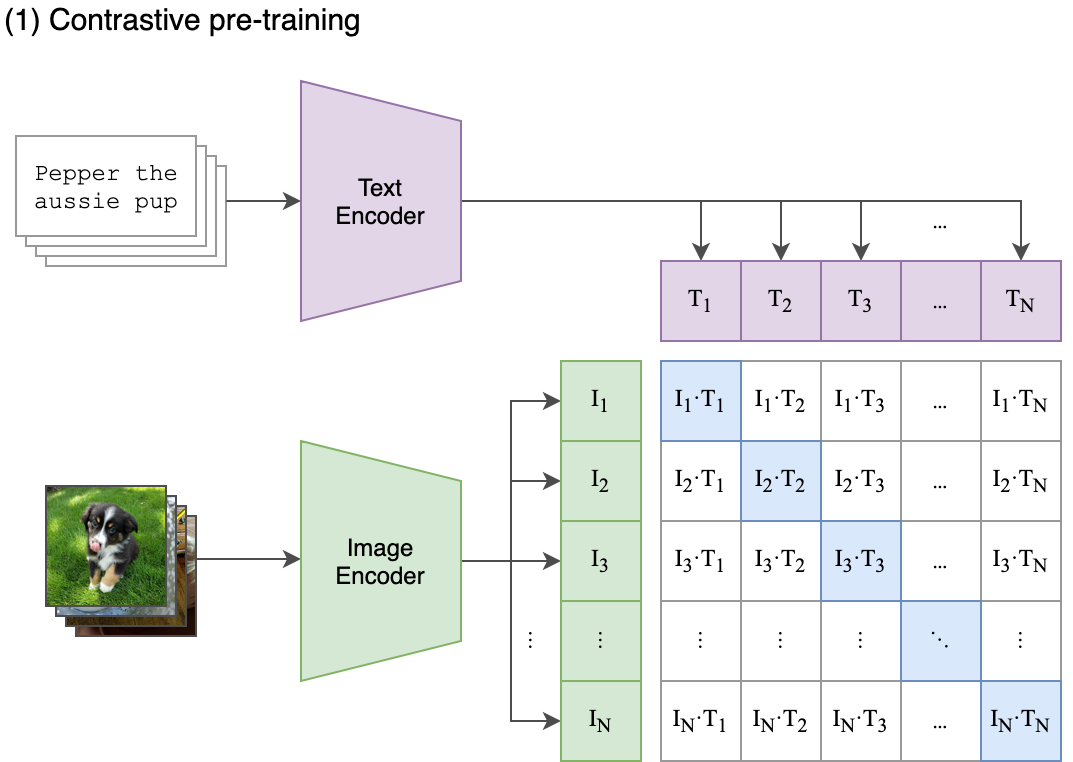
\includegraphics[width=\textwidth]{img/CLIP-structure.png}
    \caption{The CLIP model is composed by two encoders for the two visual and textual data modalities, and employs a contrastive loss function to project the input embeddings into a shared embedding space \cite{radford2021learning}.}
    \label{fig:clip}
\end{figure}

For the \emph{Text Encoder}, the authors of CLIP adopted a Transformer model \cite{vaswani2017attention} with some minor architecture modifications described in \cite{radford2019language}. The base model, that corresponds to the one used for this thesis, accounts for a size of 63M parameters, 12 layers 512-wide and 8 attention heads. For reasons of computational efficiency, the maximum sequence length accepted is capped at 76 tokens.
For the \emph{Image Encoder}, the authors of CLIP tried out two different architectures: the first is a modified version of ResNet-50 \cite{he2016deep}, inspired by the modifications done in \cite{he2019bag} and \cite{zhang2019making}, while the second is a slightly changed implementation of a Vision Transformer (ViT) \cite{dosovitskiy2020image}. The authors released checkpoints for several models belonging to both the ResNet and the ViT types. To decide which one to adopt, a careful review was conducted. In recent years, many literature works have shown  that ViTs achieve equal when not superior performance than ResNets in image classification tasks, at generally lower costs. This was demonstrated, among others, by \cite{tuli2021convolutional} who proved the superiority of ViT-B/32 versus ResNet-50 and also its higher consistency with human mistakes; by \cite{dosovitskiy2020image}, who showed how applying the Transformer architecture directly to sequences of images patches could revolutionize the field of computer vision; further confirmation of higher performance on both simple and complex tasks comes from \cite{deininger2022comparative}, \cite{hutten2022vision}, \cite{liu2024multivariate}. Soon enough, the potential of ViTs in the Remote Sensing industry started to be recognized, as shown in \cite{wang2022hyperspectral}. For these reasons, last but not least keeping in mind the most common backbones whose results are already available in the relevant literature, the ViT-B/32 has been chosen as the go-to architecture for this project and all the reported results are based on it.  

Both models are optimized during training to encode similar text and image pairs close together in a vector space shared by the two modalities, while also separating the dissimilar pairs. This means that CLIP isn't specifically trained for image classification. It was trained on a huge amount of data from the web, accounting for more than 400 million (image, text) examples; this approach was preferred to adopting an existing dataset mainly because none of them could adequately reflect the natural language variety publicly available on the internet. This dataset was constructed with the goal of covering the broadest possible set of visual concepts, whose corresponding text includes one of $500,000$ queries extracted from Wikipedia and based on word frequency. Then, they made sure there are at least $20,000$ pairs per query. The resulting dataset has a has a similar total word count as the WebText dataset used to train GPT-2. This dataset is known as \textbf{WebImageText (WIT)}.

Understanding natural language makes the model very good across different tasks, and better than traditional CNN models for generalization, and also very good at working with nuanced descriptions with higher level of detail or abstraction. These reasons are what make CLIP's zero-shot performances outstanding and why it's a very interesting model to work with.



Summary of our approach. While standard image models jointly train an image feature extractor and a linear classifier to predict
some label, CLIP jointly trains an image encoder and a text encoder to predict the correct pairings of a batch of (image, text) training
examples


CLIP \cite{radford2021learning} \\

(from CLIP's paper) \\

Looking at where zero-shot CLIP notably underperforms we see that zero-shot CLIP is quite weak on several specialized, complex, or abstract tasks such as satellite image classification (EuroSAT and RESISC45), lymph node tumor detection (PatchCamelyon), counting objects in synthetic
scenes (CLEVRCounts), self-driving related tasks such as German traffic sign recognition (GTSRB), recognizing distance to the nearest car (KITTI Distance). These results highlight the poor capability of zero-shot CLIP on more complex tasks. \\

Finally, we found that on satellite image classification datasets it helped to specify that the images were of
this form and we use variants of "a satellite photo
of a {label}."




\section{Contrastive Learning}

[Add the loss function and explain a bit how that works]

The Information Noise Contrastive Estimation (InfoNCE) loss function is a popular method for Self-Supervised Learning (SSL), and specifically Contrastive Learning (CL). In particular, CL aims at teaching the model to distinguish between similar \emph{(positive)} and dissimilar \emph{(negative)} input pairs. 


First introduced by \cite{sohn2016improved} and mostly popularized by \cite{oord2018representation}, this objective function enables CLIP to align relevant text and image input pairs by maximizing cosine similarity between matched pairs and minimizing cosine similarity for mismatches.

\section{Zero-Shot capabilities}

In computer vision, zero-shot learning usually refers to the study of generalizing to unseen object categories in image classification, that occurs when training and test classes are disjoint \cite{lampert2009learning}. However, the concept was later extended to indicate the broader case in which entire datasets are unseen.


\begin{figure}[h]
    \centering
    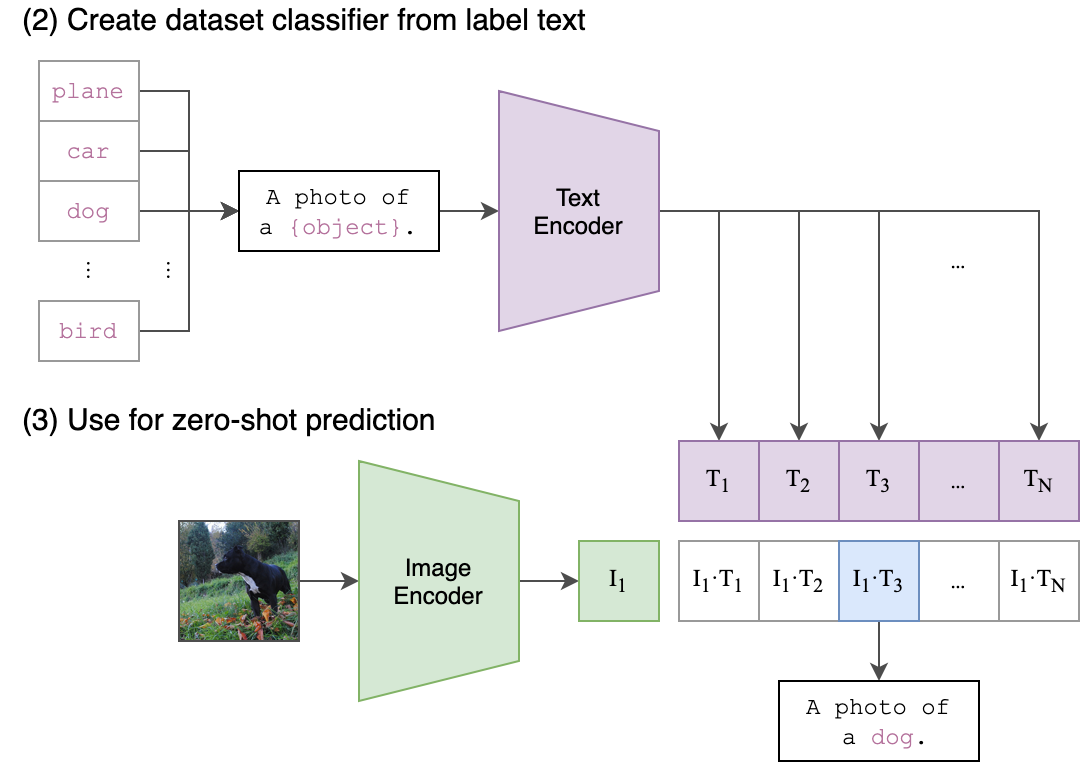
\includegraphics[width=\textwidth]{img/CLIP-zero-shot.png}
    \caption{When using CLIP for zero-shot inference, a user can feed the model custom text and image inputs and obtain similarity scores that quantify how relevant each instance of one modality is to the other.}
    \label{fig:clip-zs}
\end{figure}


\begin{figure}[h]
    \centering
    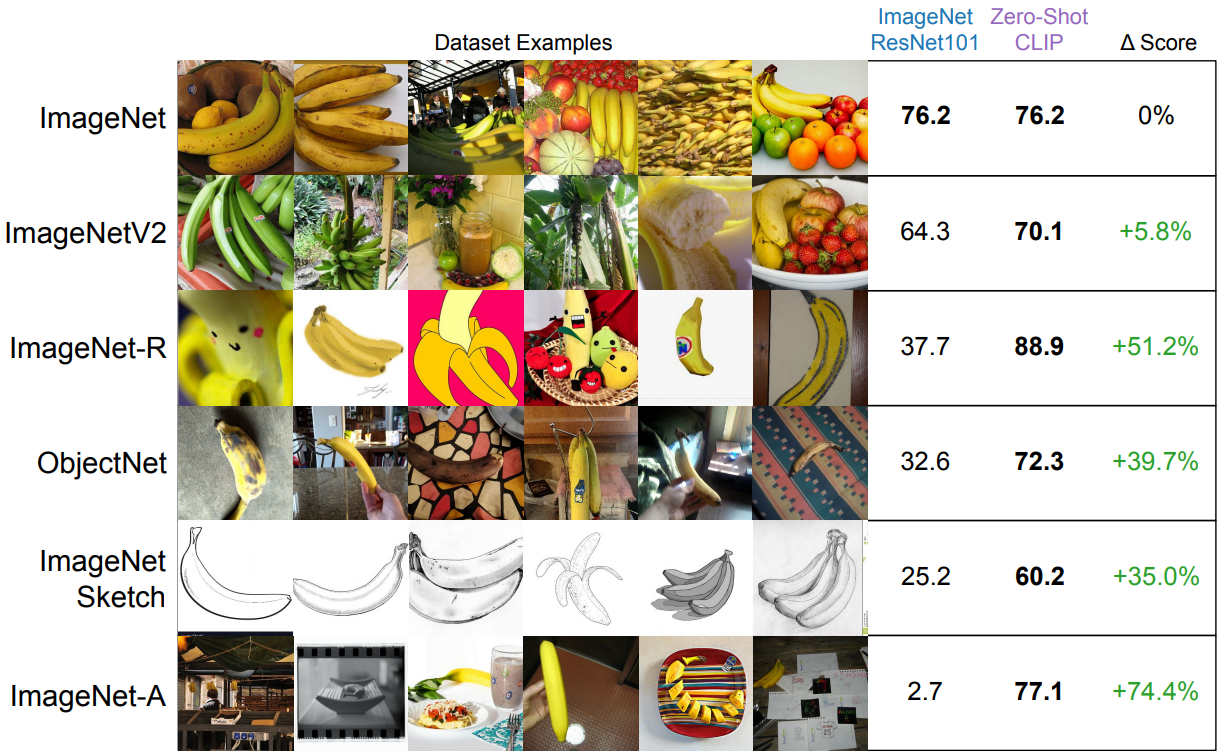
\includegraphics[width=0.7\textwidth]{img/CLIP_zero_shot.png}
    \caption{}
    \label{fig:clipzs}
\end{figure}

When the model is fed a new image-text pair, the two different modalities are processed by their corresponding encoder. Both encoders output a 512-dimensional vector.

we match the accuracy of the original ResNet-50 on ImageNet zero-shot without needing to use any of the 1.28 million training examples it was trained on.

The zero shot transfer capability of CLIP is what still today makes it an incredibly powerful and robust choice: so much so, that despite being an "old" model (released back in 2021), it's still widely adopted in both research and industry-level technology. 

Zero-shot CLIP is competitive with a fully supervised baseline


\section{CLIP-like models for Remote Sensing}

\subsection{RemoteCLIP}

\subsection{GeoRSCLIP}

\subsection{SkyCLIP}



\chapter{Datasets} % ------------------------------------------

A note before proceeding: the following datasets have been adopted due to their nature of benchmark and their importance in the literature, but they are *not* proper image-text datasets (that would be the best option to work with CLIP). This limitation is partly reflected in the final results, but they don't invalidate this work's contribution 

\section{EuroSAT}

EuroSAT \cite{helber2019eurosat} is possibly the most well known dataset in Earth Observation ground/benchmark/ studies, has been the beta-tester for all the experiments carried out in this project and the main evaluation reference to compare models performance, even if it's less diverse and comprehensive than GEO-Bench (not as complete as a benchmark) it's been around for more time and many more experiments have been carried out on it, so good for reference as well.

\begin{figure}[h]
    \centering
    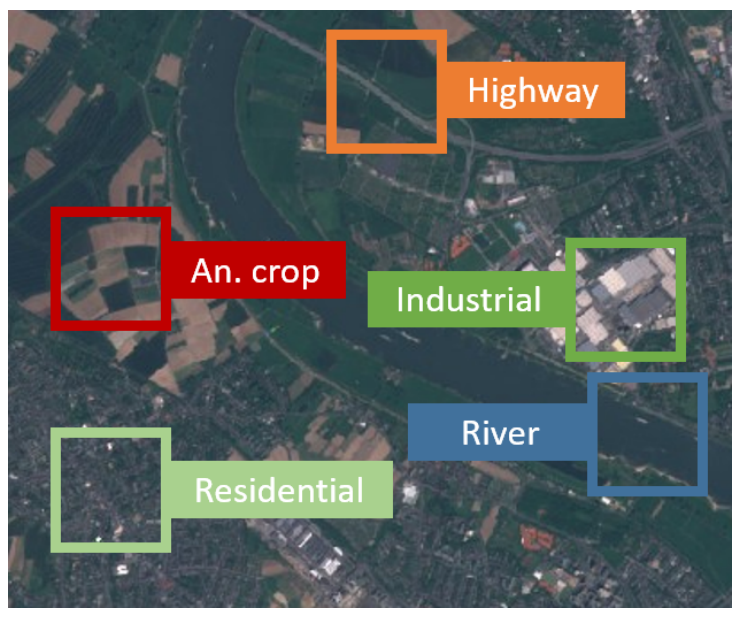
\includegraphics[width=0.5\textwidth]{img/EuroSAT_paper.png}
    \caption{Example of different patches extracted to identify different land use and land cover classes in the EuroSAT dataset.}
    \label{fig:eurosatds}
\end{figure}


\begin{figure}[h]
    \centering
    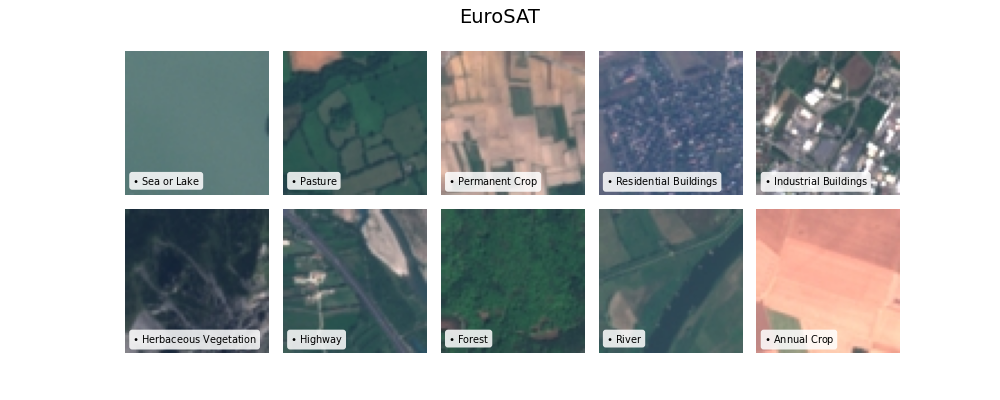
\includegraphics[width=\textwidth]{img/EuroSAT_image_grid.png}
    \caption{Sample images from the 10 classes contained in the EuroSAT original dataset.}
    \label{fig:eurosatgrid}
\end{figure}


\paragraph{Characteristics}


\begin{table}[ht]
\centering
\footnotesize
\renewcommand{\arraystretch}{1.2}
    \begin{tabular}{rcccccclcl}
    \toprule
    Name & Image Size & \# Classes & Train & Val & Test & \# Bands & RGB res & Sensors  \\
    \midrule
    EuroSAT & & 10 & 10000 & 5000 & 5000 & 13 & & Sentinel-2 \\
    \bottomrule
    \end{tabular}
\vspace{0.3cm}
\caption{\normalsize EuroSAT dataset characteristics.}
\label{tab:classtypes}
\end{table}


\begin{table}[ht]
\centering
\scriptsize
%\renewcommand{\arraystretch}{1.2}
\begin{tabular}{lccp{6cm}}  % last column for description
\toprule
\textbf{Band Name} & \textbf{Spatial} & \textbf{Central} & \textbf{Description} \\
{} & \textbf{Resolution} & \textbf{Wavelength} & \\
{} & \emph{m} & \emph{nm} & \\
\midrule
B01 - Aerosols  & 60 & 443  & Useful for atmospheric corrections and aerosol detection. \\
B02 - Blue & 10 & 490  & Penetrates water; useful for bathymetry, atmospheric corrections, and distinguishing vegetation. \\
B03 - Green & 10 & 560  & Sensitive to plant reflectance; useful for vegetation analysis and true color imagery. \\
B04 - Red & 10 & 665  & Captures vegetation and urban features; key in NDVI computation. \\
B05 - Red edge 1 & 20 & 705  & Useful for analyzing chlorophyll content and vegetation stress. \\
B06 - Red edge 2 & 20 & 740  & Enhanced vegetation sensitivity; used in crop monitoring. \\
B07 - Red edge 3 & 20 & 783  & Helps assess canopy structure and plant health. \\
B08 - NIR & 10 & 842  & Strong vegetation reflectance; essential in NDVI and biomass analysis. \\
B08A - Red edge 4 & 20 & 865  & Fills spectral gap between NIR and red edge; aids precision agriculture. \\
B09 - Water vapor & 60 & 945  & Targets atmospheric water vapor content; useful in climate and humidity studies. \\
B10 - Cirrus & 60 & 1375 & Detects high-altitude cirrus clouds; supports cloud masking. \\
B11 - SWIR 1 & 20 & 1610 & Used for vegetation moisture, snow, and burn area mapping. \\
B12 - SWIR 2 & 20 & 2190 & Helps in soil and mineral discrimination, snow and fire monitoring. \\
\bottomrule
\end{tabular}
\vspace{0.3cm}
\caption{Sentinel-2 MSI spectral bands with spatial resolution, central wavelength, and descriptive use cases.}
\label{tab:sentinel2_bands}
\end{table}


\paragraph{Composition}



\section{GEO-Bench}

The GEO-Bench dataset collection \cite{lacoste2023geo} was presented in 2023 with the purpose of .... . Its global samples span across different countries and continents, as shown in Figure \ref{fig:geoworld}. The main characteristics of the datasets of interest are summarized in the table below. 

\begin{figure}[h]
    \centering
    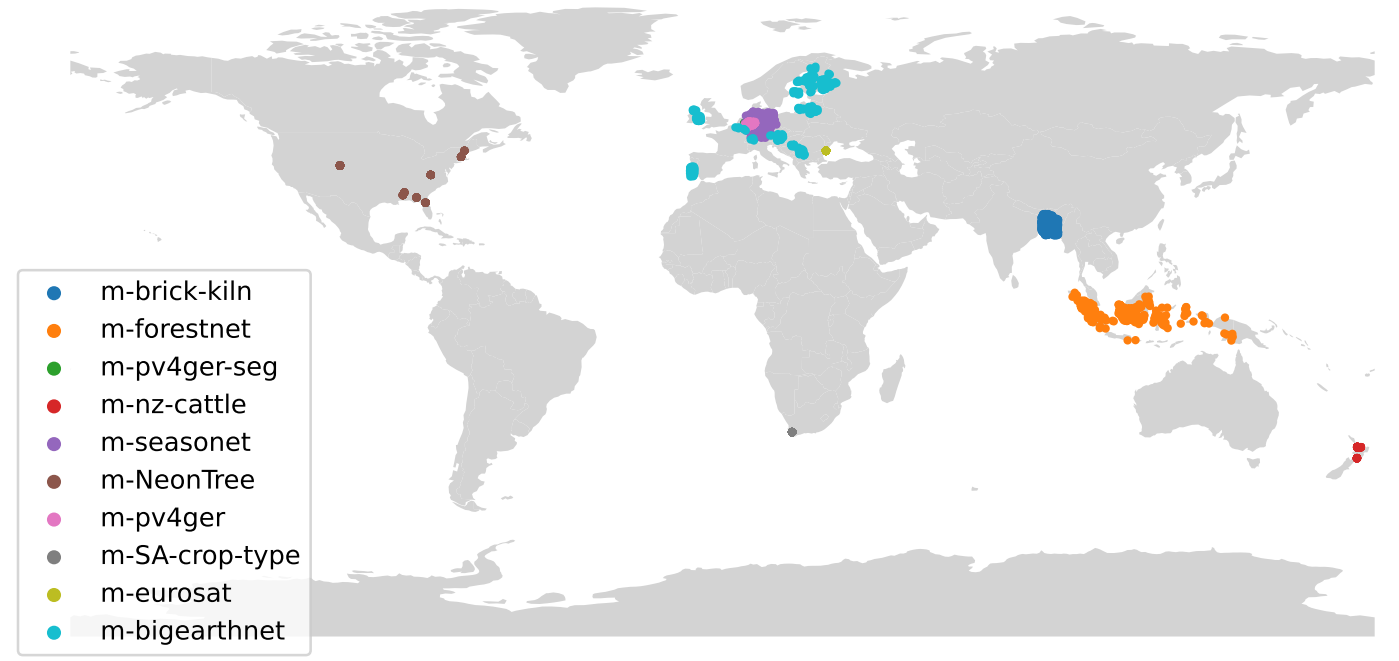
\includegraphics[width=0.6\textwidth]{img/geobench_world_coverage.png}
    \caption{The world coverage of different datasets of the benchmark, as reported in \cite{lacoste2023geo}.}
    \label{fig:geoworld}
\end{figure}

\paragraph{Composition}

The benchmark comprises six image classification datasets and six image segmentation datasets. For the purposes of this project, we will only focus on the \emph{classification} ones, a brief illustration of which follows below: \\

\begin{figure}[h]
    \centering
    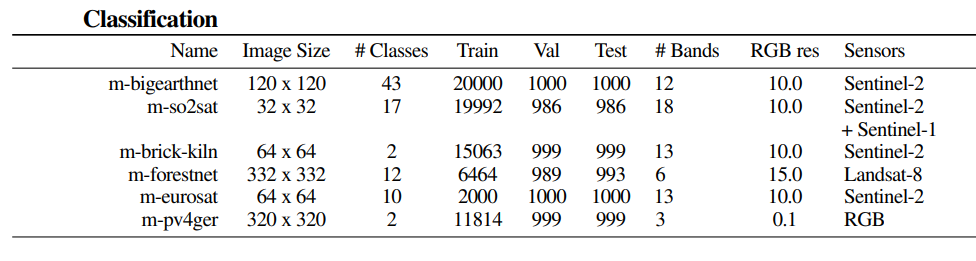
\includegraphics[width=\textwidth]{img/geobench-datasets-classification-info-cut.png}
    \caption{Characteristics of datasets in the benchmark \cite{lacoste2023geo}.}
    \label{fig:geoinfo}
\end{figure}

[List classification datasets one by one with small description, see the links in the notebook for more information and context] 


\paragraph{Diversity of Imagery} The datasets contain images acquired with different satellite sensors and preprocessed by different technologies, resulting in images with different size, resolution, and available spectral bands.


\paragraph{Diversity of Classification Tasks} The classification datasets are the result of different studies conducted with different purposes, therefore they are associated to a different kind of classification tasks. Except for the binary case, the other tasks vary greatly in number and type of classes, and these differences are outlined in Table \ref{tab:classtypes}. Here, "short captions" identifies class names identified by $2-3$ words at most, while "caption" refers to class names identified by $>5$ words, and "words" trivially refers to class names identified by single words.


\begin{table}[ht]
\centering
\footnotesize
\renewcommand{\arraystretch}{1.2}
    \begin{tabular}{lcccc}
    \toprule
    \textbf{Dataset} & \textbf{Origin} & \textbf{Classification task} & \textbf{\# Classes} & \textbf{Type of classes}  \\
    \midrule
    m-brick-kiln & GEO-Bench & binary & 2 & short captions \\
    m-pv4ger & GEO-Bench & binary & 2 & short captions \\
    m-forestnet & GEO-Bench & multiclass & 12 & words \\
    m-eurosat & GEO-Bench & multiclass & 10 & words \\
    m-so2sat & GEO-Bench & multiclass & 17 & words \\
    m-bigearthnet & GEO-Bench & multilabel & 43 & captions \\
    \bottomrule
    \end{tabular}
\vspace{0.3cm}
\caption{\normalsize Classification task details for every dataset analyzed.}
\label{tab:classtypes}
\end{table}


\subsection{m-brick-kiln}


\begin{figure}[h]
    \centering
    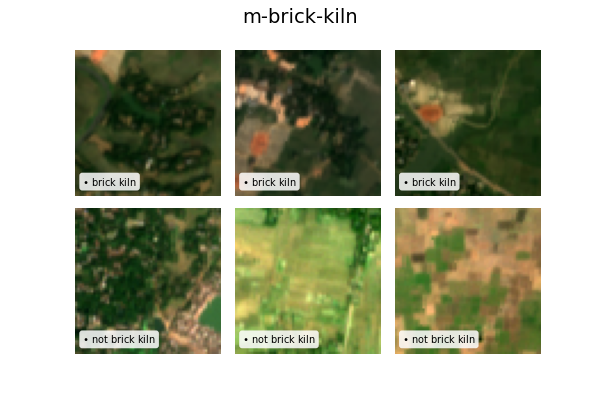
\includegraphics[width=0.7\textwidth]{img/m-brick-kiln_image_grid.png}
    \caption{Sample images from the 2 classes contained in the m-brick-kiln dataset from GEO-Bench.}
    \label{fig:brickgrid}
\end{figure}


\subsection{m-pv4ger}

\begin{figure}[h]
    \centering
    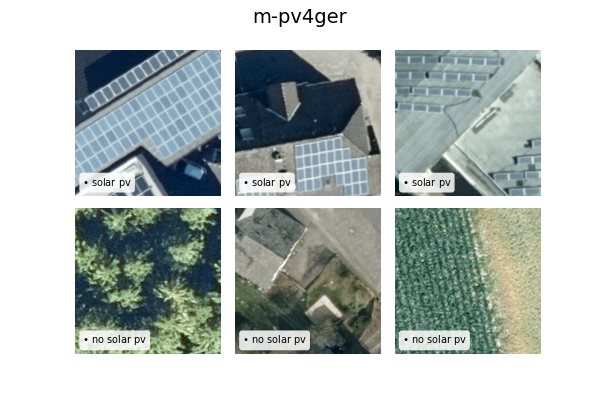
\includegraphics[width=0.7\textwidth]{img/m-pv4ger_image_grid.png}
    \caption{Sample images from the 2 classes contained in the m-pv4ger dataset from GEO-Bench.}
    \label{fig:solargrid}
\end{figure}


\subsection{m-forestnet}


\begin{figure}[h]
    \centering
    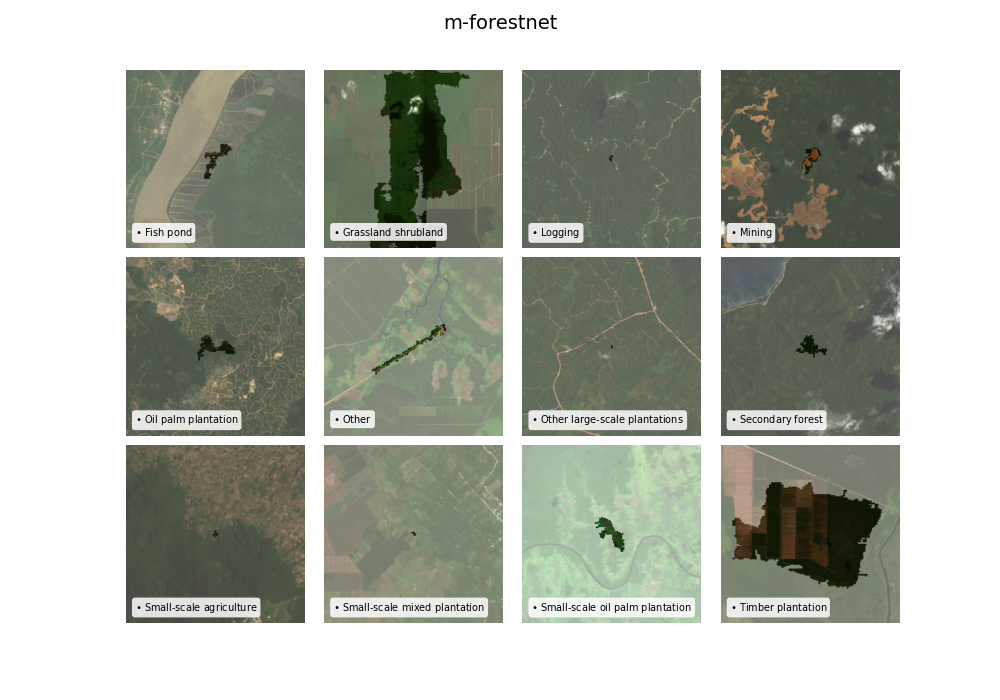
\includegraphics[width=0.8\textwidth]{img/m-forestnet_image_grid.png}
    \caption{Sample images from the 12 classes contained in the m-forestnet dataset from GEO-Bench.}
    \label{fig:forestnetgrid}
\end{figure}


\subsection{m-eurosat}

Specify how this dataset was preprocessed and modified, highlight differences wrt the original EuroSAT


\begin{figure}[h]
    \centering
    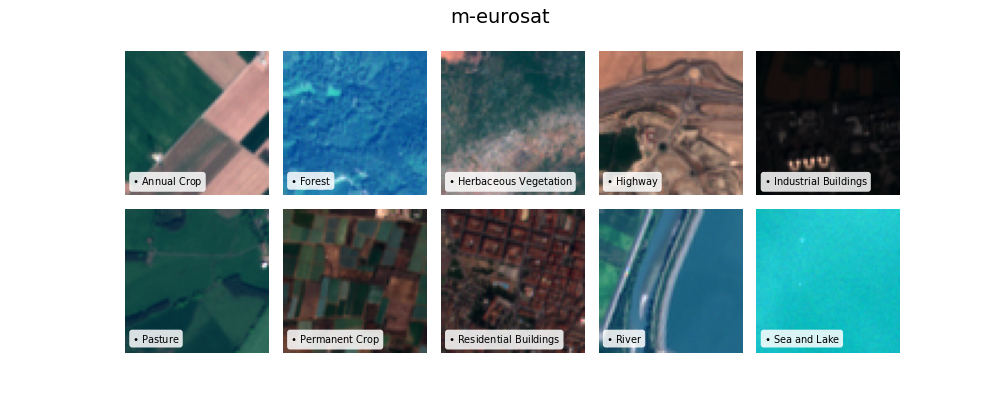
\includegraphics[width=\textwidth]{img/m-eurosat_image_grid.png}
    \caption{Sample images from the 10 classes contained in the m-eurosat dataset from GEO-Bench.}
    \label{fig:meurosatgrid}
\end{figure}


\subsection{m-so2sat}


\begin{figure}[h]
    \centering
    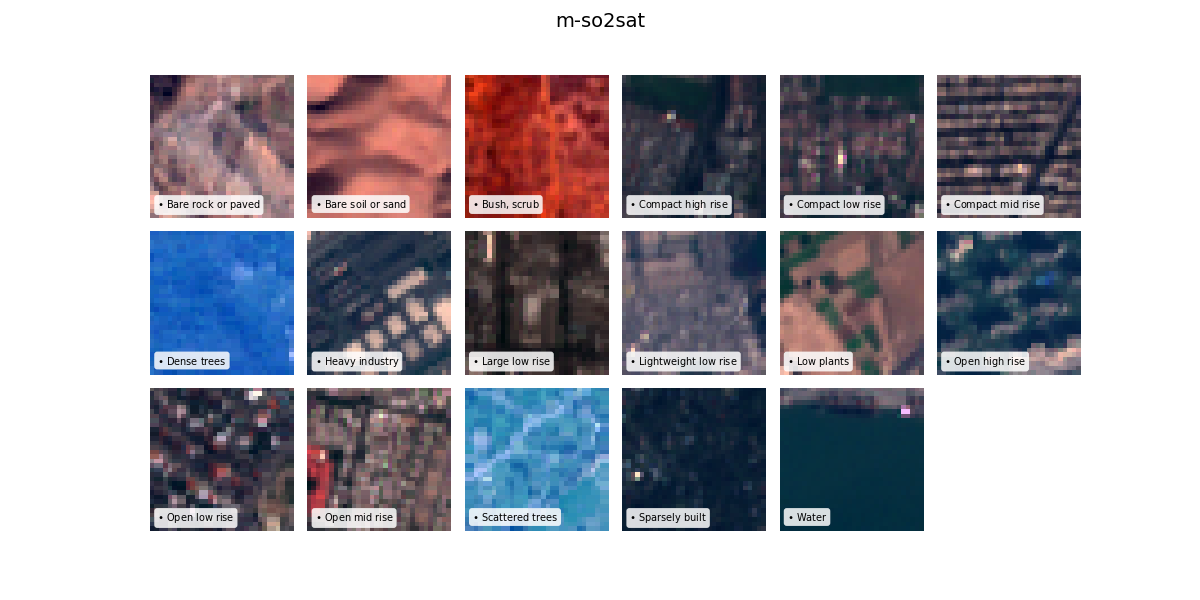
\includegraphics[width=\textwidth]{img/m-so2sat_image_grid.png}
    \caption{Sample images from the 17 classes contained in the m-so2sat dataset from GEO-Bench.}
    \label{fig:so2satgrid}
\end{figure}


\subsection{m-bigearthnet}


\begin{figure}[h]
    \centering
    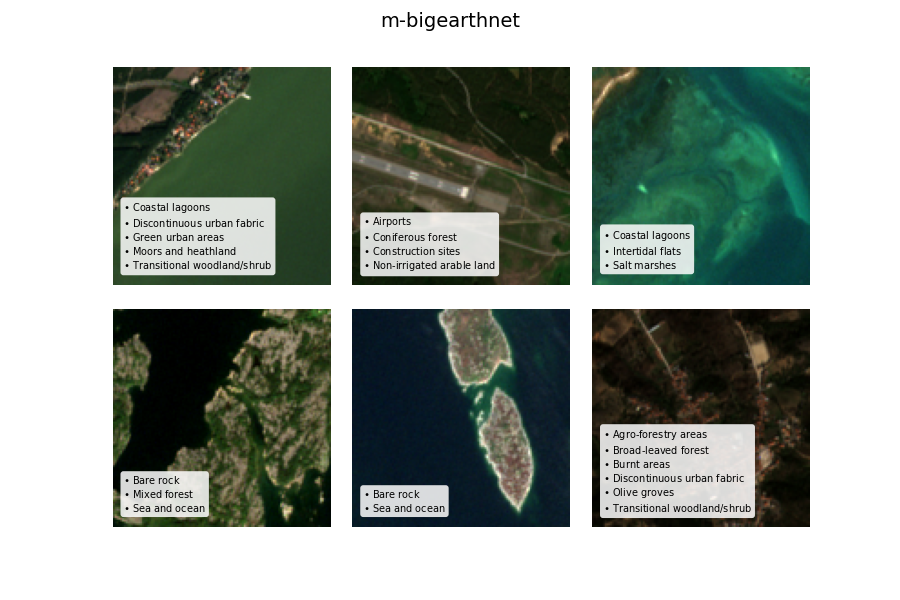
\includegraphics[width=\textwidth]{img/m-bigearthnet_image_grid.png}
    \caption{Sample multilabel images featured in the m-bigearthnet dataset from GEO-Bench.}
    \label{fig:bengrid}
\end{figure}


\chapter{Approach} % ------------------------------------------

\section{Multi Spectral Embedders}

(Explain the concept)


\subsection{MSI-1 embedder}

(add some pseudocode)

\subsection{MSI-2 embedder}
\subsection{MSI-T embedder}

\section{MSI + CLIP Model Structure}

(add a schematization of where the embedder is placed in the model)

\paragraph{Base model}

(how the model works for specific datasets, adapting to the number of available bands, training and testing for the specific case)

\paragraph{Transfer Learning model}

(how the embedder trained on a specific dataset (and how that dataset was chosen) 

\chapter{Experimental setup} % --------------------------------

This project focuses on some ground benchmarking work in the scope of \emph{image classification}. This task has been chosen for reasons like a lack of baseline results to compare CLIP-like models to different types of VLMs, but also between themselves. Given the versatility of these models and the possible application to several types of tasks, the literature disagrees/is not uniform in the tasks (and consequentially in the evaluation) of these models. For simplicity, and to make the results more significant in the context of existing literature, and to fill small research gaps that miss a comprehensive evaluation of these models, we choose here to focus on classification (also for the "universality" of this task, it's easy to understand, it's easy to compare models on it). Therefore, we adopt the classic classification evaluation metrics for the binary and multiclass tasks, while some more research has been carried out to evaluate the multilabel task as it needs to be treated a bit differently.

\section{Evaluation metrics}

\paragraph{Binary/Multiclass Classification}

\begin{itemize}
    \item \textbf{Accuracy}:
    \item \textbf{Precision}:
    \item \textbf{Recall}:
    \item \textbf{F1 Score}:
    \item \textbf{Confusion Matrix}
\end{itemize}

\paragraph{Multilabel Classification}

\begin{itemize}
    \item \textbf{Precision@k (P@k)}:
    \item \textbf{Recall@k (R@k)}:
    \item \textbf{Mean Average Precision (mAP)}:
    \item \textbf{Micro F1}:
    \item \textbf{Ranking Loss}:
\end{itemize}


\section{Baseline tests}

\paragraph{EuroSAT}

\begin{table}[h]
\centering
\footnotesize
\renewcommand{\arraystretch}{1.2}
    \begin{tabular}{llc}
    \specialrule{.1em}{.2em}{.2em}
    \textbf{Model} & \textbf{Backbone} & \textbf{EuroSAT} \\
    \specialrule{.06em}{.2em}{.2em}
    CLIP        & ViT-B/32 & 38.76\% \\ 
    RemoteCLIP  & ViT-B/32 & 37.34\% \\
    GeoRSCLIP   & ViT-B/32 & \textbf{53.54\%} \\
    SkyCLIP     & ViT-B/32 & 52.26\% \\
    \specialrule{.1em}{.2em}{.2em}
    \end{tabular}
\vspace{0.3cm}
\caption{\normalsize Comparison of zero-shot accuracies obtained by different models on the EuroSAT original dataset.}
\label{tab:eurobaselines}
\end{table}


\begin{figure}[h]
  \begin{subfigure}[t]{.5\textwidth}
    \centering
    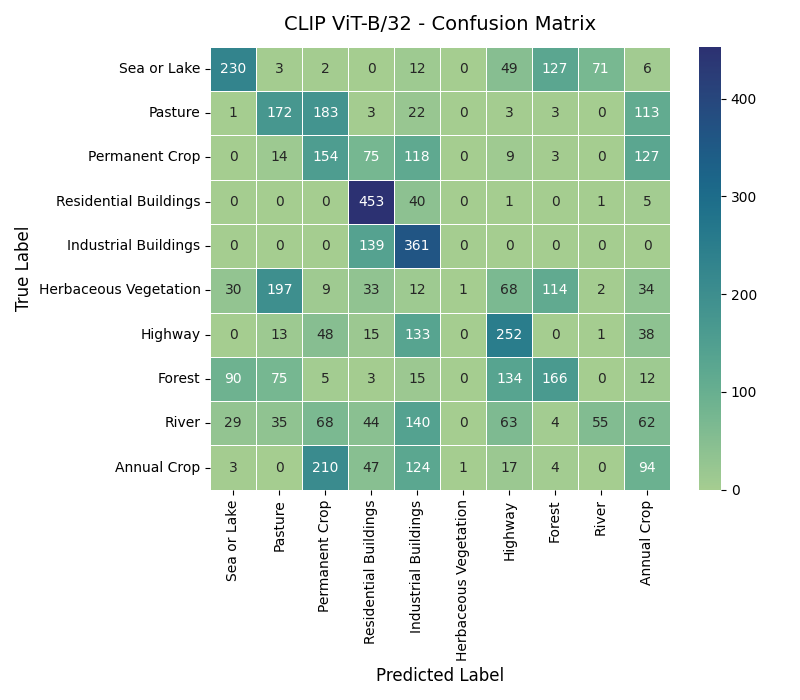
\includegraphics[width=\linewidth]{img/EuroSAT_CLIP_32_cm.png}
    %\caption{}
  \end{subfigure}
  \hfill
  \begin{subfigure}[t]{.5\textwidth}
    \centering
    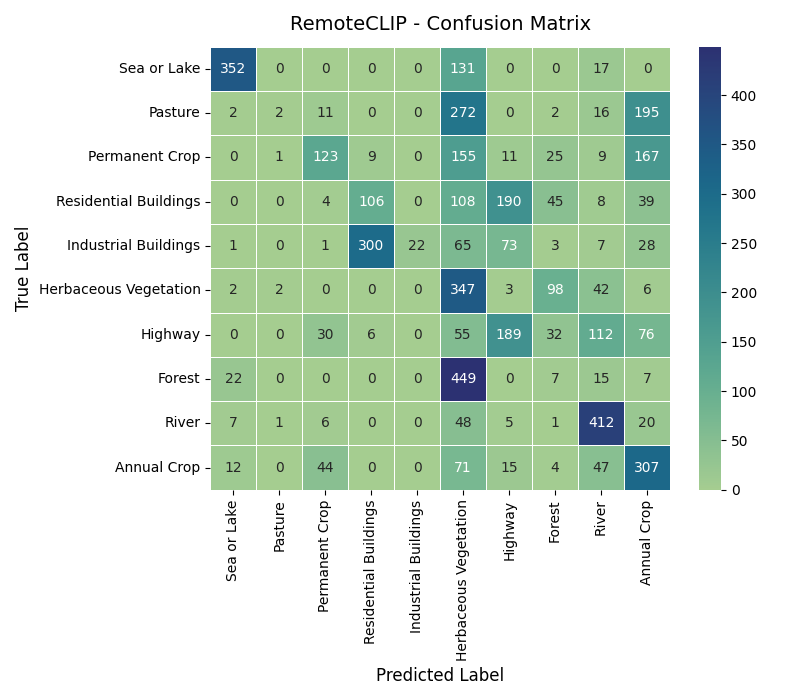
\includegraphics[width=\linewidth]{img/EuroSAT_RemoteCLIP_32_cm.png}
    %\caption{}
  \end{subfigure}

  \medskip

  \begin{subfigure}[t]{.5\textwidth}
    \centering
    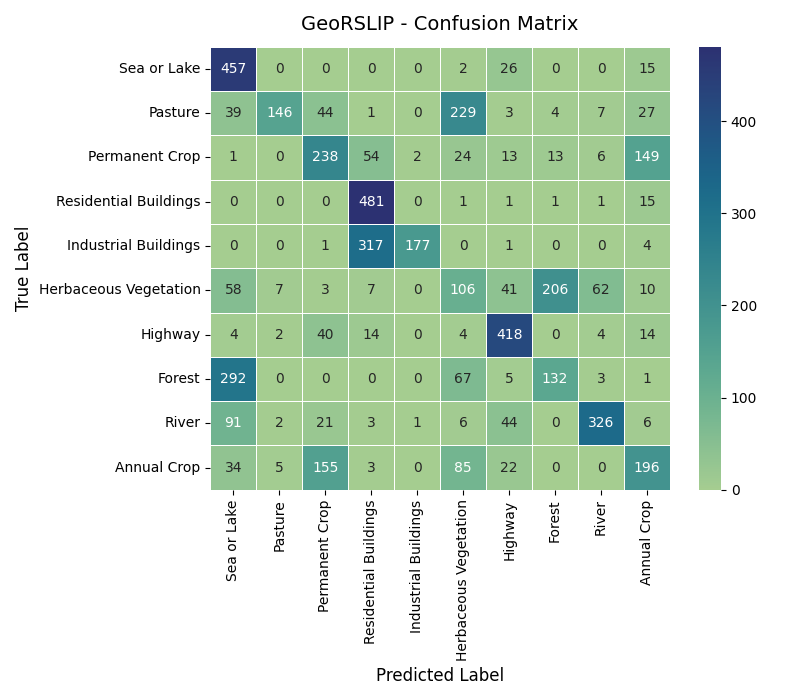
\includegraphics[width=\linewidth]{img/EuroSAT_GeoRSCLIP_32_cm.png}
    %\caption{}
  \end{subfigure}
  \hfill
  \begin{subfigure}[t]{.5\textwidth}
    \centering
    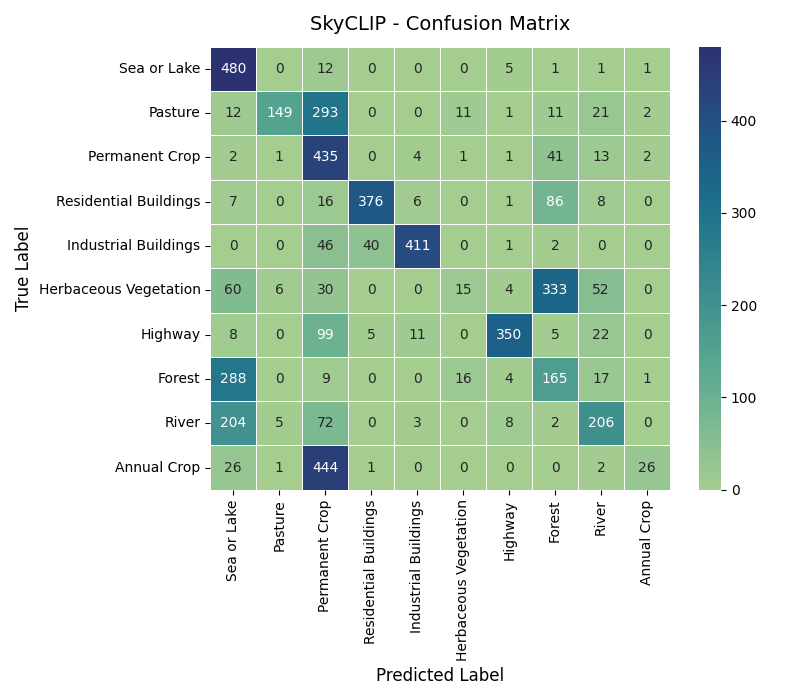
\includegraphics[width=\linewidth]{img/EuroSAT_SkyCLIP_32_cm.png}
    %\caption{}
  \end{subfigure}
  \caption{Confusion matrices of CLIP and other CLIP-like models finetuned on Remote Sensing datasets, evaluated on EuroSAT: while CLIP and RemoteCLIP's matrices appear somewhat fuzzy and struggle to recognize some classes at all, GeoRSCLIP and SkyCLIP's ones feature a more definite diagonal.}
\end{figure}



\paragraph{GEO-Bench}


\begin{table}[ht]
\centering
\footnotesize
\renewcommand{\arraystretch}{1.2}
    \begin{tabular}{llccccc}
    %\hline
    \specialrule{.1em}{.2em}{.2em}
    \textbf{Model} & \textbf{Backbone} & \textbf{m-brick-kiln} & \textbf{m-pv4ger} & \textbf{m-forestnet} & \textbf{m-eurosat} & \textbf{m-so2sat} \\
    %{} & {} & \textbf{acc} & \textbf{acc} & \textbf{acc} & \textbf{acc} & \textbf{acc} \\
    %\hline
    \specialrule{.06em}{.2em}{.2em}
    CLIP        & ViT-B/32 & \textbf{70.27\%} & 73.87\% & 7.65\% & 41.90\% & \textbf{16.63\%}\\ %\hdashline[2pt/5pt]
    RemoteCLIP  & ViT-B/32 & 66.97\% & 65.97\% & 8.25\% & 28.70\% & 12.78\% \\
    GeoRSCLIP   & ViT-B/32 & 68.67\% & 89.09\% & \textbf{14.20\%} & \textbf{51.30\%} & 15.82\% \\
    SkyCLIP     & ViT-B/32 & 59.36\% & \textbf{90.59\%} & 10.67\% & 49.30\% & 12.27\% \\
    %\hline
    \specialrule{.1em}{.2em}{.2em}
    \end{tabular}
\vspace{0.3cm}
\caption{\normalsize Comparison of zero-shot accuracies obtained by different models across GEO-Bench datasets.}
\label{tab:baselines}
\end{table}


\begin{table}[ht]
\centering
\footnotesize
\renewcommand{\arraystretch}{1.2}
    \begin{tabular}{llcccc|c}
    \toprule
    %\textbf{Model} & \textbf{Method} & \multicolumn{5}{c}{\textbf{m-bigearthnet}} \\
    \multirow{2}{*}{\textbf{Model}} & \multirow{2}{*}{\textbf{Backbone}} & \multicolumn{5}{c}{\textbf{m-bigearthnet}} \\
    \cmidrule(lr){3-7}
    & & \textbf{R@5} & \textbf{P@5} & \textbf{mAP} & \textbf{F1} & \textbf{rloss} \\
    \specialrule{.06em}{.2em}{.2em}
    CLIP        & ViT-B/32 & 31.70\% & 23.40\% & 32.32\% & 20.39\% & 28.71\% \\ 
    RemoteCLIP  & ViT-B/32 & 26.24\% & 19.82\% & 27.63\%  & 20.30\% & 30.89\%  \\
    GeoRSCLIP   & ViT-B/32 & \textbf{38.89\%} & \textbf{28.60\%} & \textbf{39.69\%} & 22.15\% & \textbf{23.19\%} \\
    SkyCLIP     & ViT-B/32 & 26.53\% & 19.30\% & 28.61\% & \textbf{22.39\%} & 30.98\%  \\
    \bottomrule
    \end{tabular}
\vspace{0.3cm}
\caption{\normalsize Comparison of zero-shot performance metrics obtained by different models on the m-bigearthnet dataset from GEO-Bench.}
\label{tab:baselines-multilab}
\end{table}


\section{Text prompts experiments}

* Focus on binary classification *

- Explain the problems with negation, cite paper \cite{quantmeyer2024and}

- Explain the idea behind the binary approach and the one behind the multi-prompt approach

(from CLIP's original paper, valid not only for text prompts experiment but also baseline tests)

Another issue we encountered is that it’s relatively rare in our pre-training dataset for the text paired with the image to be just a single word. Usually the text is a full sentence describing the image in some way. To help bridge this distribution gap, we found that using the prompt template “A photo of a {label}.” to be a good default that helps specify the text is about the content of the image. This often improves performance over the baseline of using only the label text.

Finally, we found that on satellite image classification datasets it helped to specify that the images were of this form and we use variants of “a satellite photo of a {label}.”.


\paragraph{m-brick-kiln}

TODO: List the prompts and the corresponding mapping to positive/negative classes


\begin{table}[ht]
\centering
\footnotesize
\renewcommand{\arraystretch}{1.2}
    \begin{tabular}{lc|cccc}
    \toprule
    %\textbf{Model} & \textbf{original} & \textbf{Prompt 1} & \textbf{Prompt 2} & \textbf{Prompt 3} & \textbf{Multi-Prompt} \\
    \multirow{2}{*}{\textbf{Model}} & \multicolumn{4}{c}{\textbf{Binary Prompts}} &  \multirow{2}{*}{\textbf{Multi-Prompt}}\\
    \cmidrule(lr){2-5}
    & \textbf{Original} & \textbf{Type 1} & \textbf{Type 2} & \textbf{Type 3} \\
    \midrule
    CLIP & 70.27\% & 76.58\% & 80.38\% & 79.78\% & \textbf{83.58\%} \\
    RemoteCLIP & 66.97\% & 66.27\% & 66.77\% & \textbf{67.47\%} & 66.57\% \\
    GeoRSCLIP & 68.67\% & 71.87\% & 70.57\% & \textbf{73.37\%} & 68.17\%\\
    SkyCLIP & 59.36\% & 69.07\% & \textbf{69.27\%} & 69.17\% & 67.57\% \\ 
    \bottomrule
    \end{tabular}
\vspace{0.3cm}
\caption{\normalsize CLIP performance on m-brick-kiln with different text prompts.}
\label{tab:prompts1}
\end{table}


\paragraph{m-pv4ger}

TODO: List the prompts and the corresponding mapping to positive/negative classes


\begin{table}[ht]
\centering
\footnotesize
\renewcommand{\arraystretch}{1.2} % increase row spacing
    \begin{tabular}{lc|cccc}
    \toprule
    %\textbf{Model} & \textbf{original} & \textbf{Prompt 1} & \textbf{Prompt 2} & \textbf{Prompt 3} & \textbf{Multi-Prompt} \\
    \multirow{2}{*}{\textbf{Model}} & \multicolumn{4}{c}{\textbf{Binary Prompts}} &  \multirow{2}{*}{\textbf{Multi-Prompt}}\\
    \cmidrule(lr){2-5}
    & \textbf{Original} & \textbf{Type 1} & \textbf{Type 2} & \textbf{Type 3} \\
    \midrule
    CLIP & 73.87\% & 71.57\% & 79.28\% & 76.78\% & \textbf{82.88\%} \\
    RemoteCLIP & 65.97\% & 45.85\% & 48.15\% & 32.03\% & \textbf{74.47\%} \\
    GeoRSCLIP & 89.09\% & \textbf{94.19\%} & 93.29\% & 93.89\% & 92.09\% \\
    SkyCLIP & 90.59\% & 91.99\% & 90.79\% & 91.59\% & \textbf{92.09\%} \\
    \bottomrule
    \end{tabular}
\vspace{0.3cm}
\caption{\normalsize CLIP performance on m-pv4ger with different text prompts.}
\label{tab:prompts2}
\end{table}


\section{Image normalization experiments}

\begin{figure}[h]
    \centering
    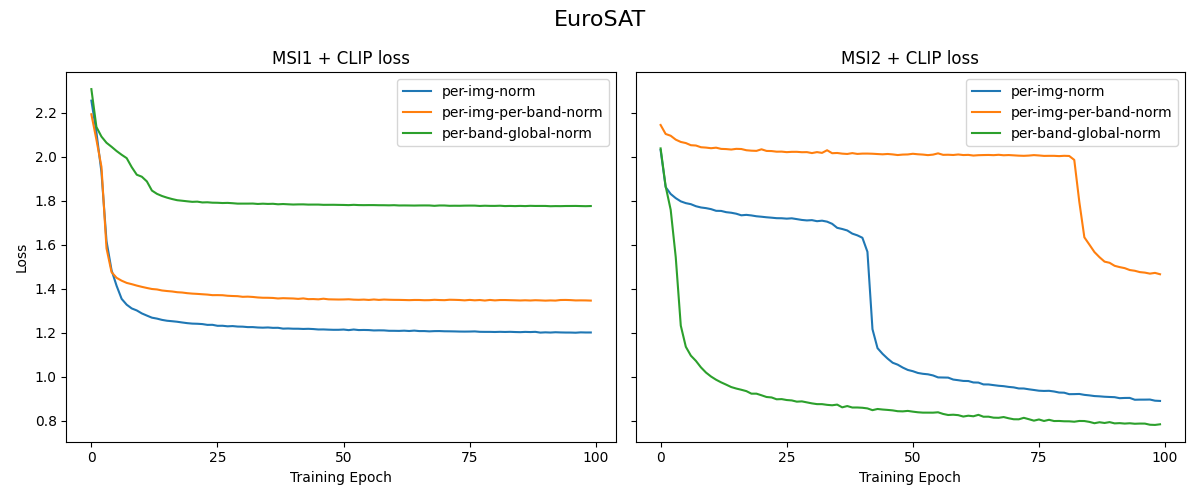
\includegraphics[width=\textwidth]{img/EuroSAT_norm_losses_plot.png}
    \caption{The effect of different normalization functions on the convergence of the training loss for the two different models.}
    \label{fig:normlosses}
\end{figure}

- comments of what normalization works best for the different models, how we calculated them, lin min max, cite \cite{unknown}, etc - 

Mention that to keep integrity and consistency with the dataset we adopt norm3 for all the following experiments and training.


\chapter{Results} % -------------------------------------------

\section{Finetuning results}


\paragraph{EuroSAT}


\begin{table}[h]
\centering
\footnotesize
\renewcommand{\arraystretch}{1.2}
    \begin{tabular}{ccc}
    \specialrule{.1em}{.2em}{.2em}
    \textbf{Model} & \textbf{Method} & \textbf{EuroSAT} \\
    \specialrule{.06em}{.2em}{.2em}
    CLIP        & zero-shot & 38.76\% \\ 
    | &  | & | \\
    MSI1+CLIP & MSI1 training  & 37.29\% \\
    {} & $\pm\Delta$ & \textcolor{red}{-1.47\%} \\
    MSI2+CLIP & MSI2 training & \textbf{75.44\%} \\
    {} & $\pm\Delta$ & \textcolor{customgreen}{+36.68\%} \\
    \specialrule{.1em}{.2em}{.2em}
    \end{tabular}
\vspace{0.3cm}
\caption{\normalsize Comparison of accuracies obtained after training different embedders on the EuroSAT original dataset: the first embedder almost matches the zero shot performance, while the second nearly doubles it.}
\label{tab:eurobaselines}
\end{table}



\paragraph{GEO-Bench}


\begin{table}[ht]
\centering
\footnotesize
\renewcommand{\arraystretch}{1.3} 
    \begin{tabular}{ccccccc}
    %\hline
    \specialrule{.1em}{.2em}{.2em}
    \textbf{Model} & \textbf{Method} & \textbf{m-brick-kiln} & \textbf{m-pv4ger} & \textbf{m-forestnet} & \textbf{m-eurosat} & \textbf{m-so2sat} \\
    %\hline
    \specialrule{.06em}{.2em}{.2em}
    CLIP      & zero-shot & 70.27\% & 73.87\% & 7.65\% & 41.90\% & \underline{16.63\%} \\
    | &  | & | & | & | &| & | \\
    MSI1+CLIP & MSI1 training & \underline{86.38\%} & \underline{92.19\%} & \textbf{10.67\%} & 44.40\% & 15.82\% \\
    {} & $\pm\Delta$ & \textcolor{customgreen}{+16.11\%} & \textcolor{customgreen}{+18.32\%} & \textcolor{customgreen}{+3.02\%} & \textcolor{customgreen}{+2.50\%} & \textcolor{red}{-0.81\%} \\
    MSI2+CLIP & MSI2 training & \textbf{90.19\%} & \textbf{92.89\%} & \underline{9.86\%} & \textbf{67.50\%} & \textbf{18.45\%} \\
    {} & $\pm\Delta$ & \textcolor{customgreen}{+19.92\%} & \textcolor{customgreen}{+19.02} & \textcolor{customgreen}{+2.21\%} & \textcolor{customgreen}{+25.60\%} & \textcolor{customgreen}{+1.82\%} \\
    \specialrule{.1em}{.2em}{.2em}
    \end{tabular}
\vspace{0.3cm}
\caption{\normalsize Comparison of models with respect to the original CLIP, after training the embedders: the score in bold refers to the best model and the underlined one to the second best.}
\label{tab:msimodels}
\end{table}



\section{Transfer Learning results}

\begin{table}[ht]
\centering
\footnotesize
\renewcommand{\arraystretch}{1.3} 
    \begin{tabular}{ccccccc}
    %\hline
    \specialrule{.1em}{.2em}{.2em}
    \textbf{Model} & \textbf{Method} & \textbf{m-brick-kiln} & \textbf{m-pv4ger} & \textbf{m-forestnet} & \textbf{m-eurosat} & \textbf{m-so2sat} \\
    %\hline
    \specialrule{.06em}{.2em}{.2em}
    CLIP      & zero-shot & \textbf{70.27\%} & \underline{73.87\%} & 7.65\% & 41.90\% & \underline{16.63\%} \\
    | &  | & | & | & | &| & | \\
    MSI-T-s & zero shot & 56.35\% & 71.97\% & 8.76\% & 16.79\% & \textbf{20.08\%} \\
    (m-so2sat train) & $\pm\Delta$ & \textcolor{red}{-13.92\%} & \textcolor{red}{-1.90\%} & \textcolor{customgreen}{+1.11\%} & \textcolor{red}{-25.11\%} & \textcolor{customgreen}{+3.45\%} \\
    %\specialrule{.01em}{.2em}{.2em}
    MSI-T-E & zero shot & 62.46\% & 53.25\% & \underline{10.27\%} & \underline{46.79\%} & 9.43\% \\
    (EuroSAT train) & $\pm\Delta$ & \textcolor{red}{-7.81\%} & \textcolor{red}{-20.62\%} & \textcolor{customgreen}{+2.62\%} & \textcolor{customgreen}{+4.89\%} & \textcolor{red}{-7.20\%} \\
    %\specialrule{.01em}{.2em}{.2em}
     MSI-T-E-4L & zero shot & \underline{69.36\%} & \textbf{86.68\%} & \textbf{11.48\%} & \textbf{53.60\%} &  5.88\% \\
    (EuroSAT train) & $\pm\Delta$ & \textcolor{red}{-0.91\%} & \textcolor{customgreen}{+12.81\%} & \textcolor{customgreen}{+3.83\%} & \textcolor{customgreen}{+11.70\%} & \textcolor{red}{-10.75\%} \\
    %\hline
    \specialrule{.1em}{.2em}{.2em}
    \end{tabular}
\vspace{0.3cm}
\caption{\normalsize Comparison of models with respect to the original CLIP: the accuracy in bold refers to the best performing model, the underlined one to the second best.}
\label{tab:msimodels}
\end{table}




% Loss plots
\begin{figure}[h]
    \centering
    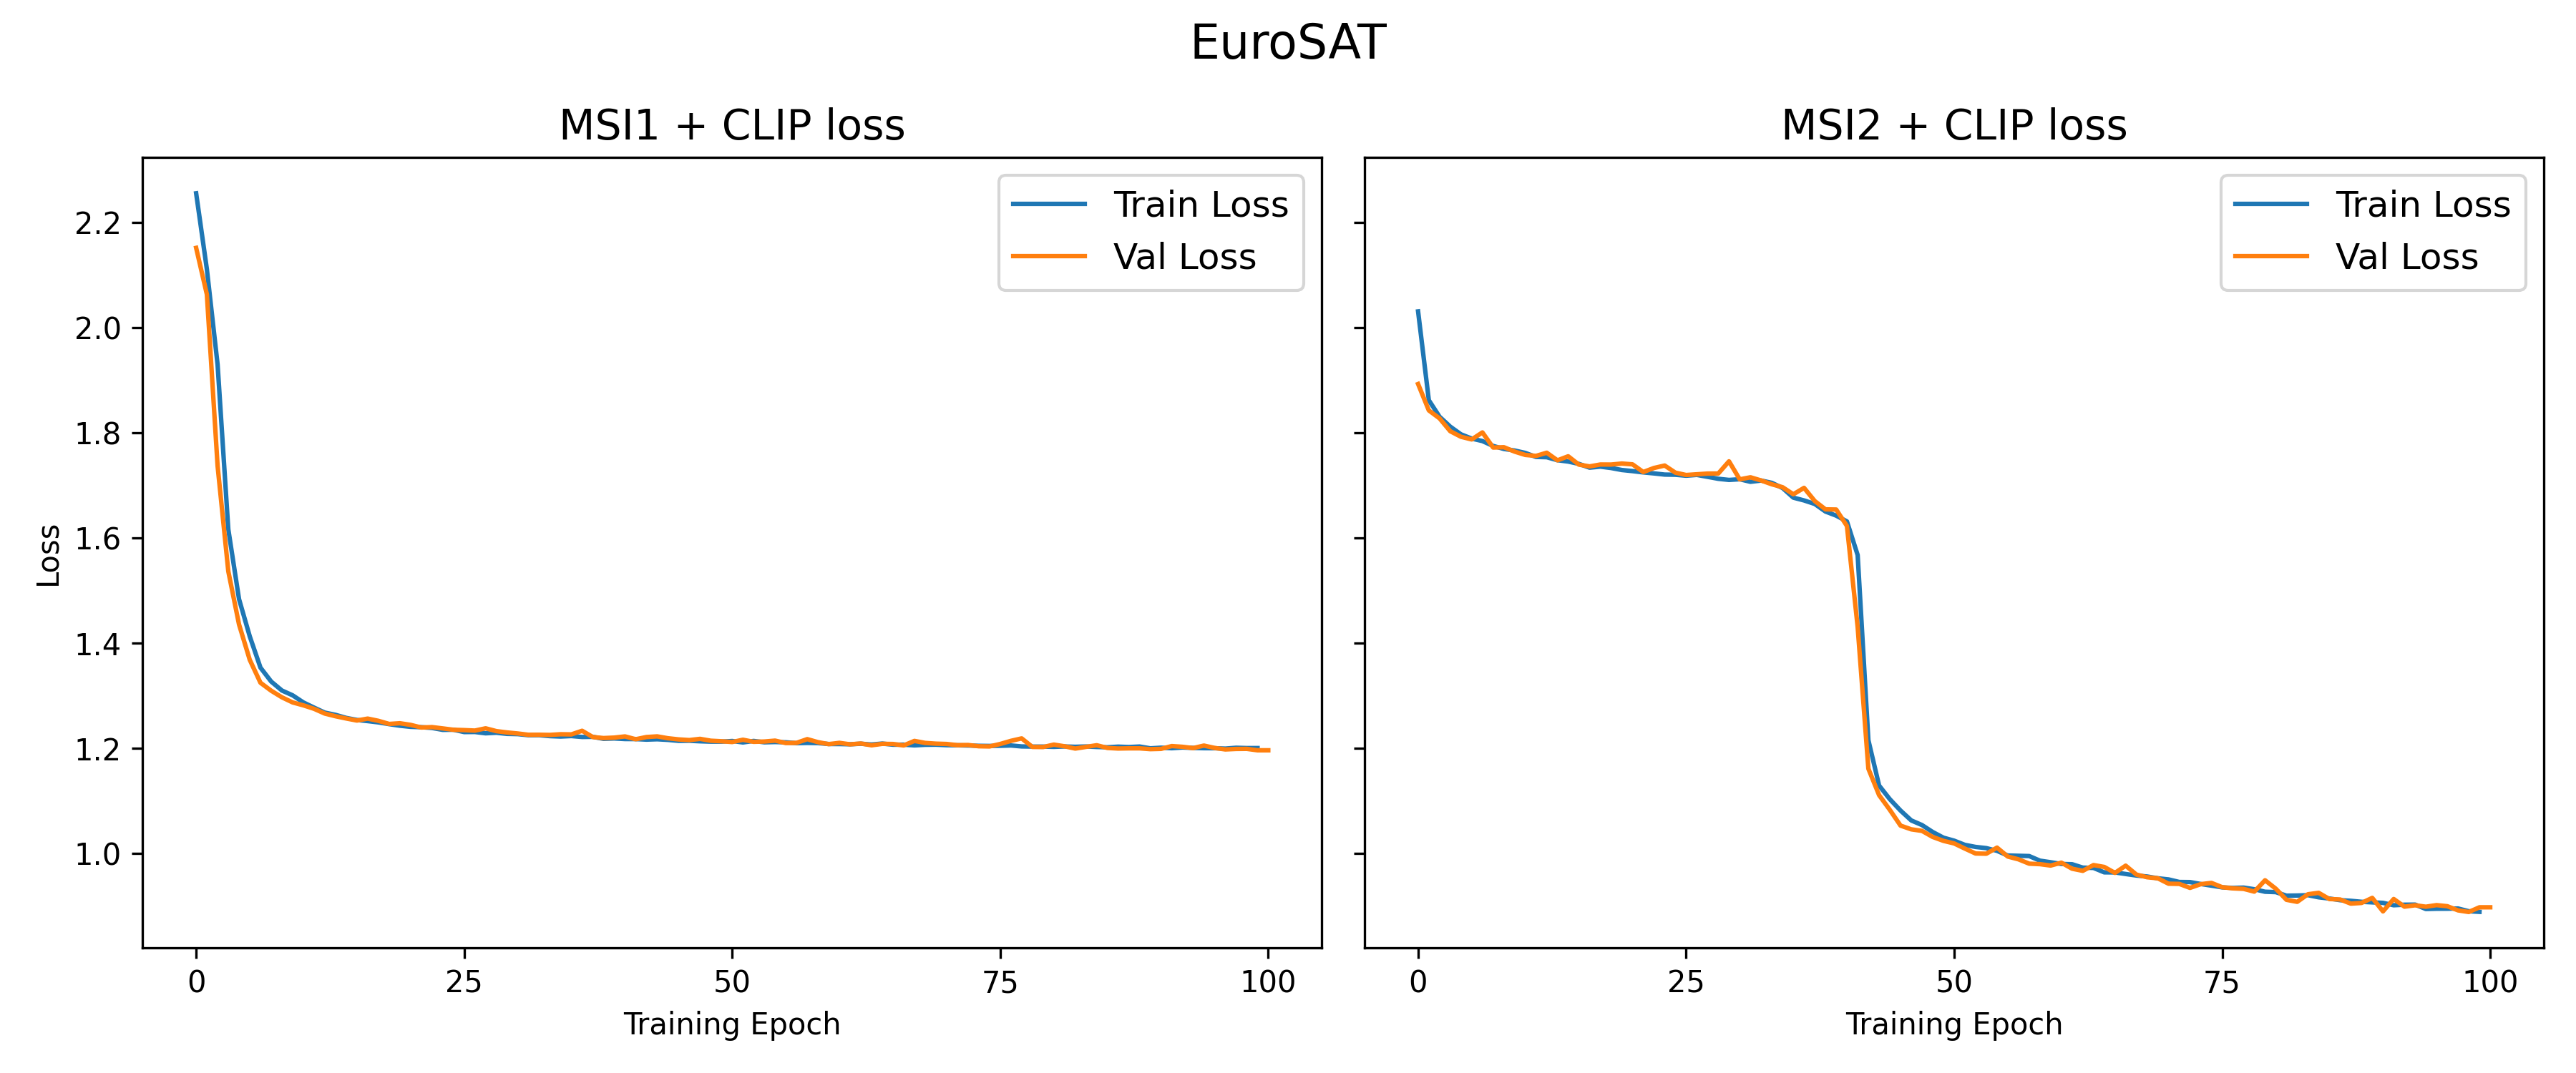
\includegraphics[width=\textwidth]{img/EuroSAT_loss_plot.png}
    \caption{Training and validation loss of the two embedders on the original EuroSAT dataset.}
    \label{fig:eurosatloss}
\end{figure}


\begin{figure}[h]
    \centering
    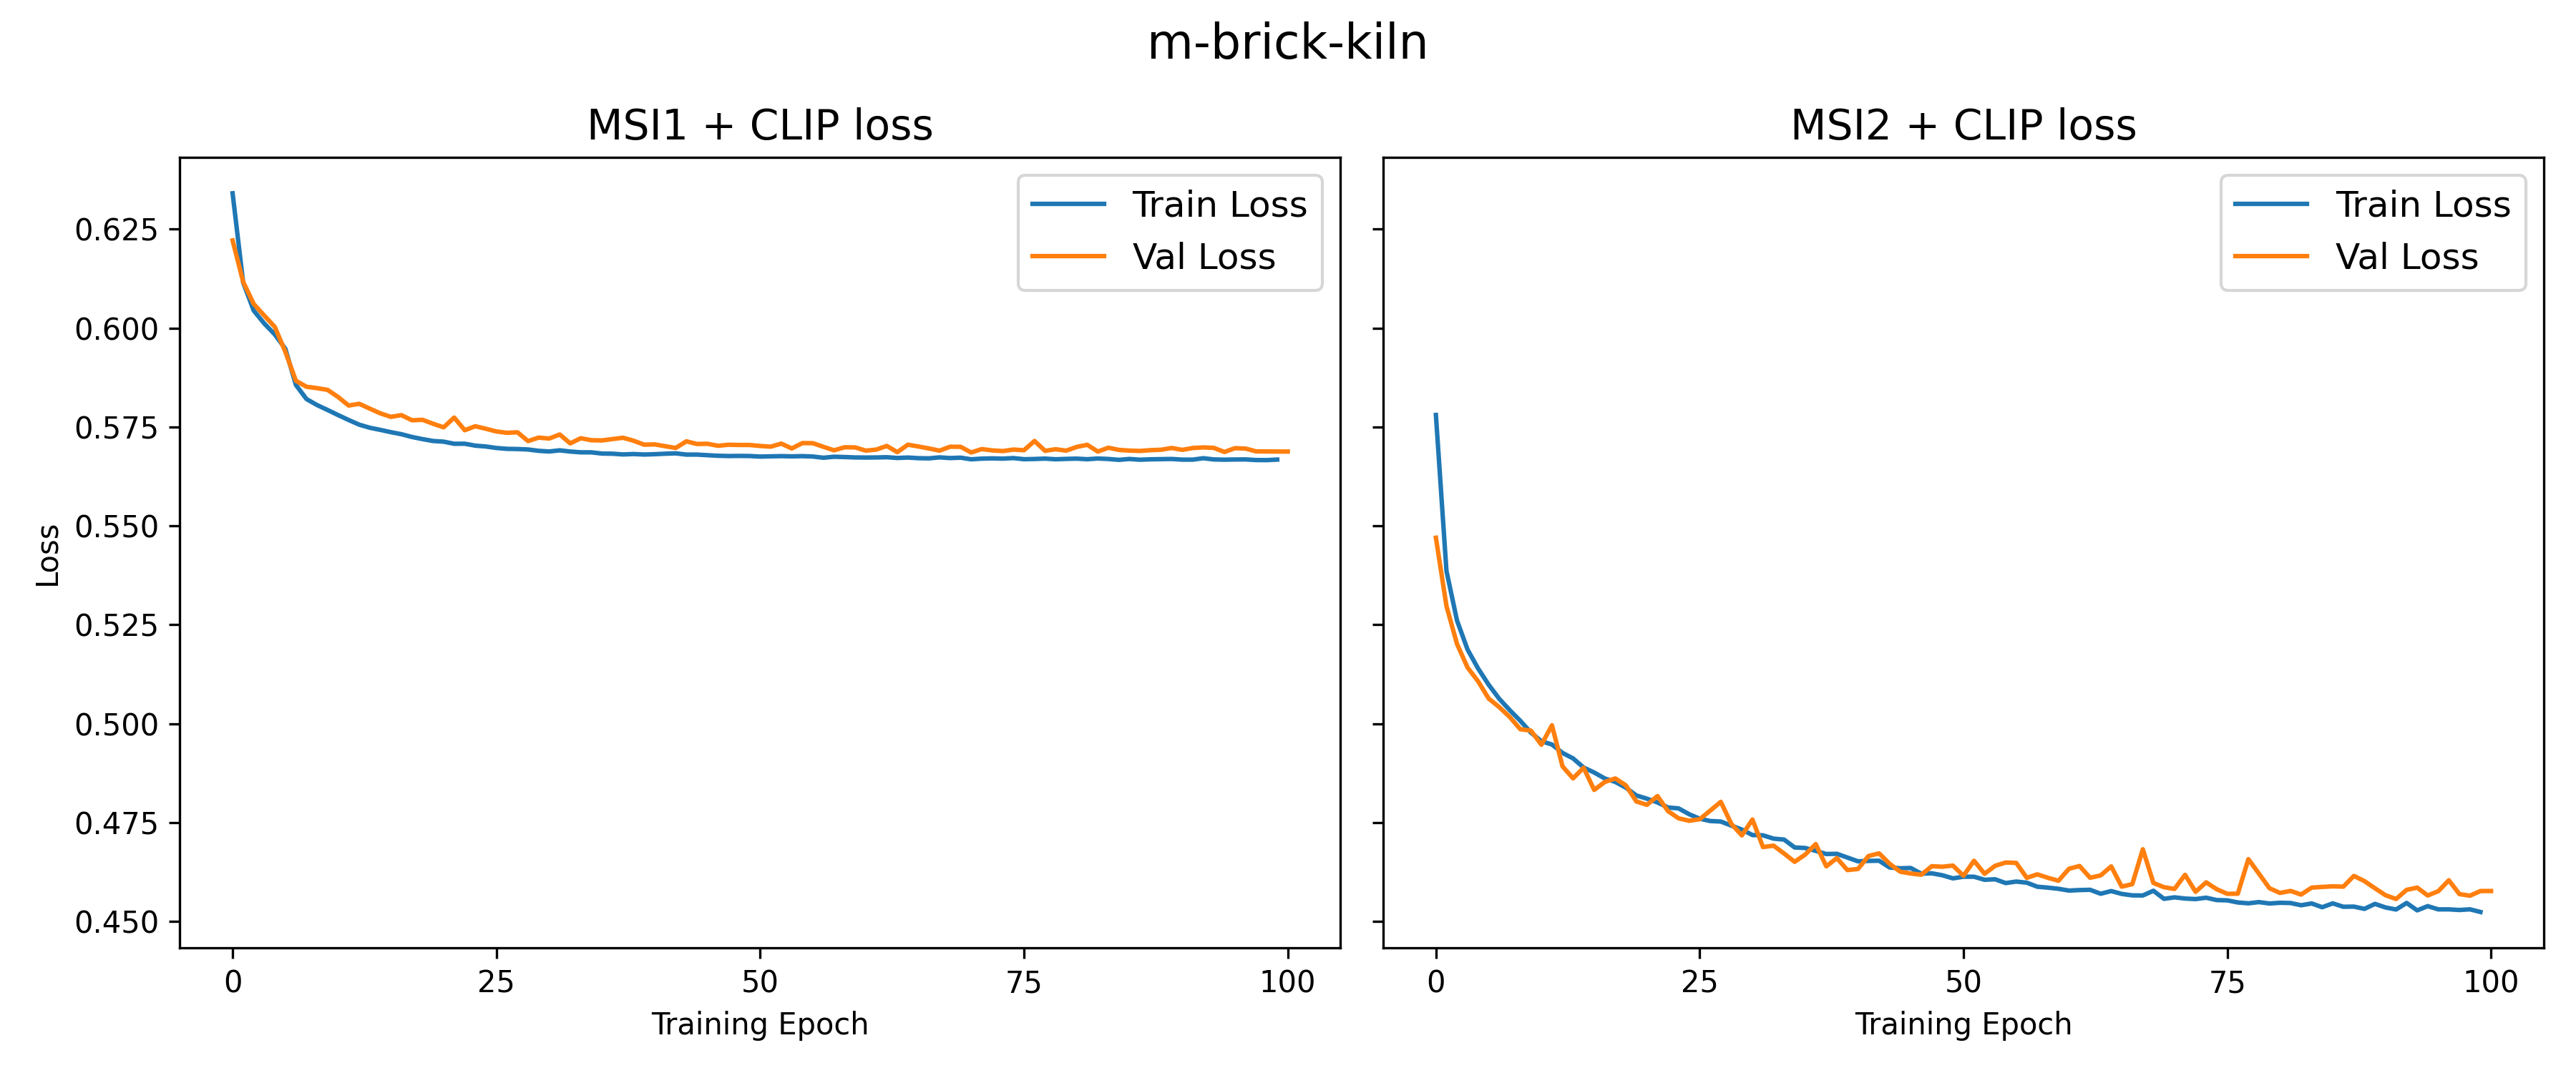
\includegraphics[width=\textwidth]{img/m-brick-kiln_loss_plot.png}
    \caption{Training and validation loss of the two embedders on the m-brick-kiln dataset from GEO-Bench.}
    \label{fig:brickloss}
\end{figure}

\begin{figure}[h]
    \centering
    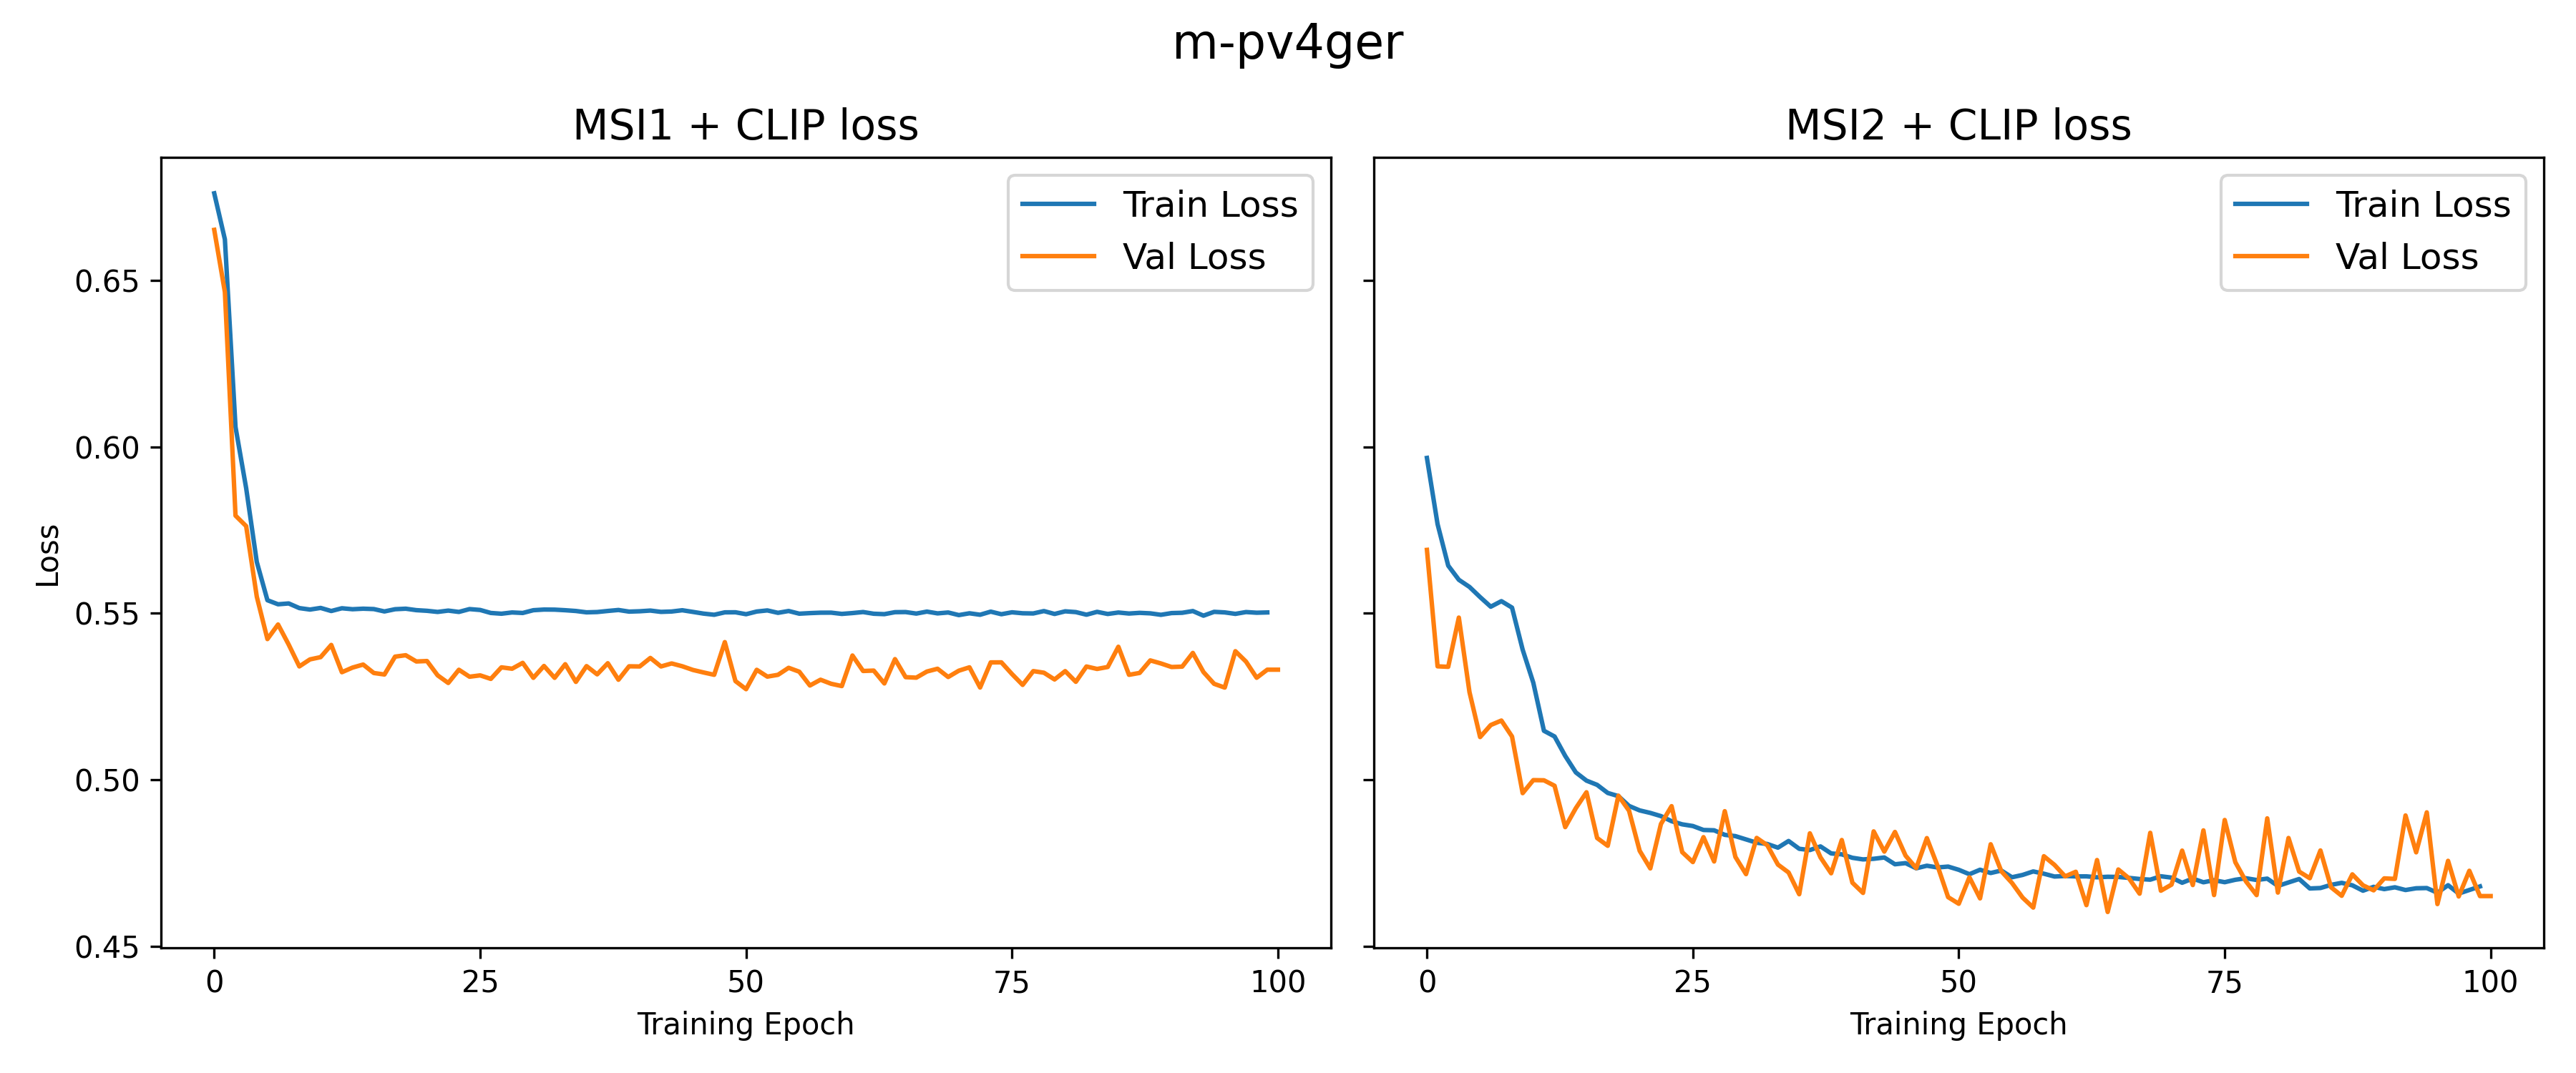
\includegraphics[width=\textwidth]{img/m-pv4ger_loss_plot.png}
    \caption{Training and validation loss of the two embedders on the m-pv4ger dataset from GEO-Bench.}
    \label{fig:solarloss}
\end{figure}

\begin{figure}[h]
    \centering
    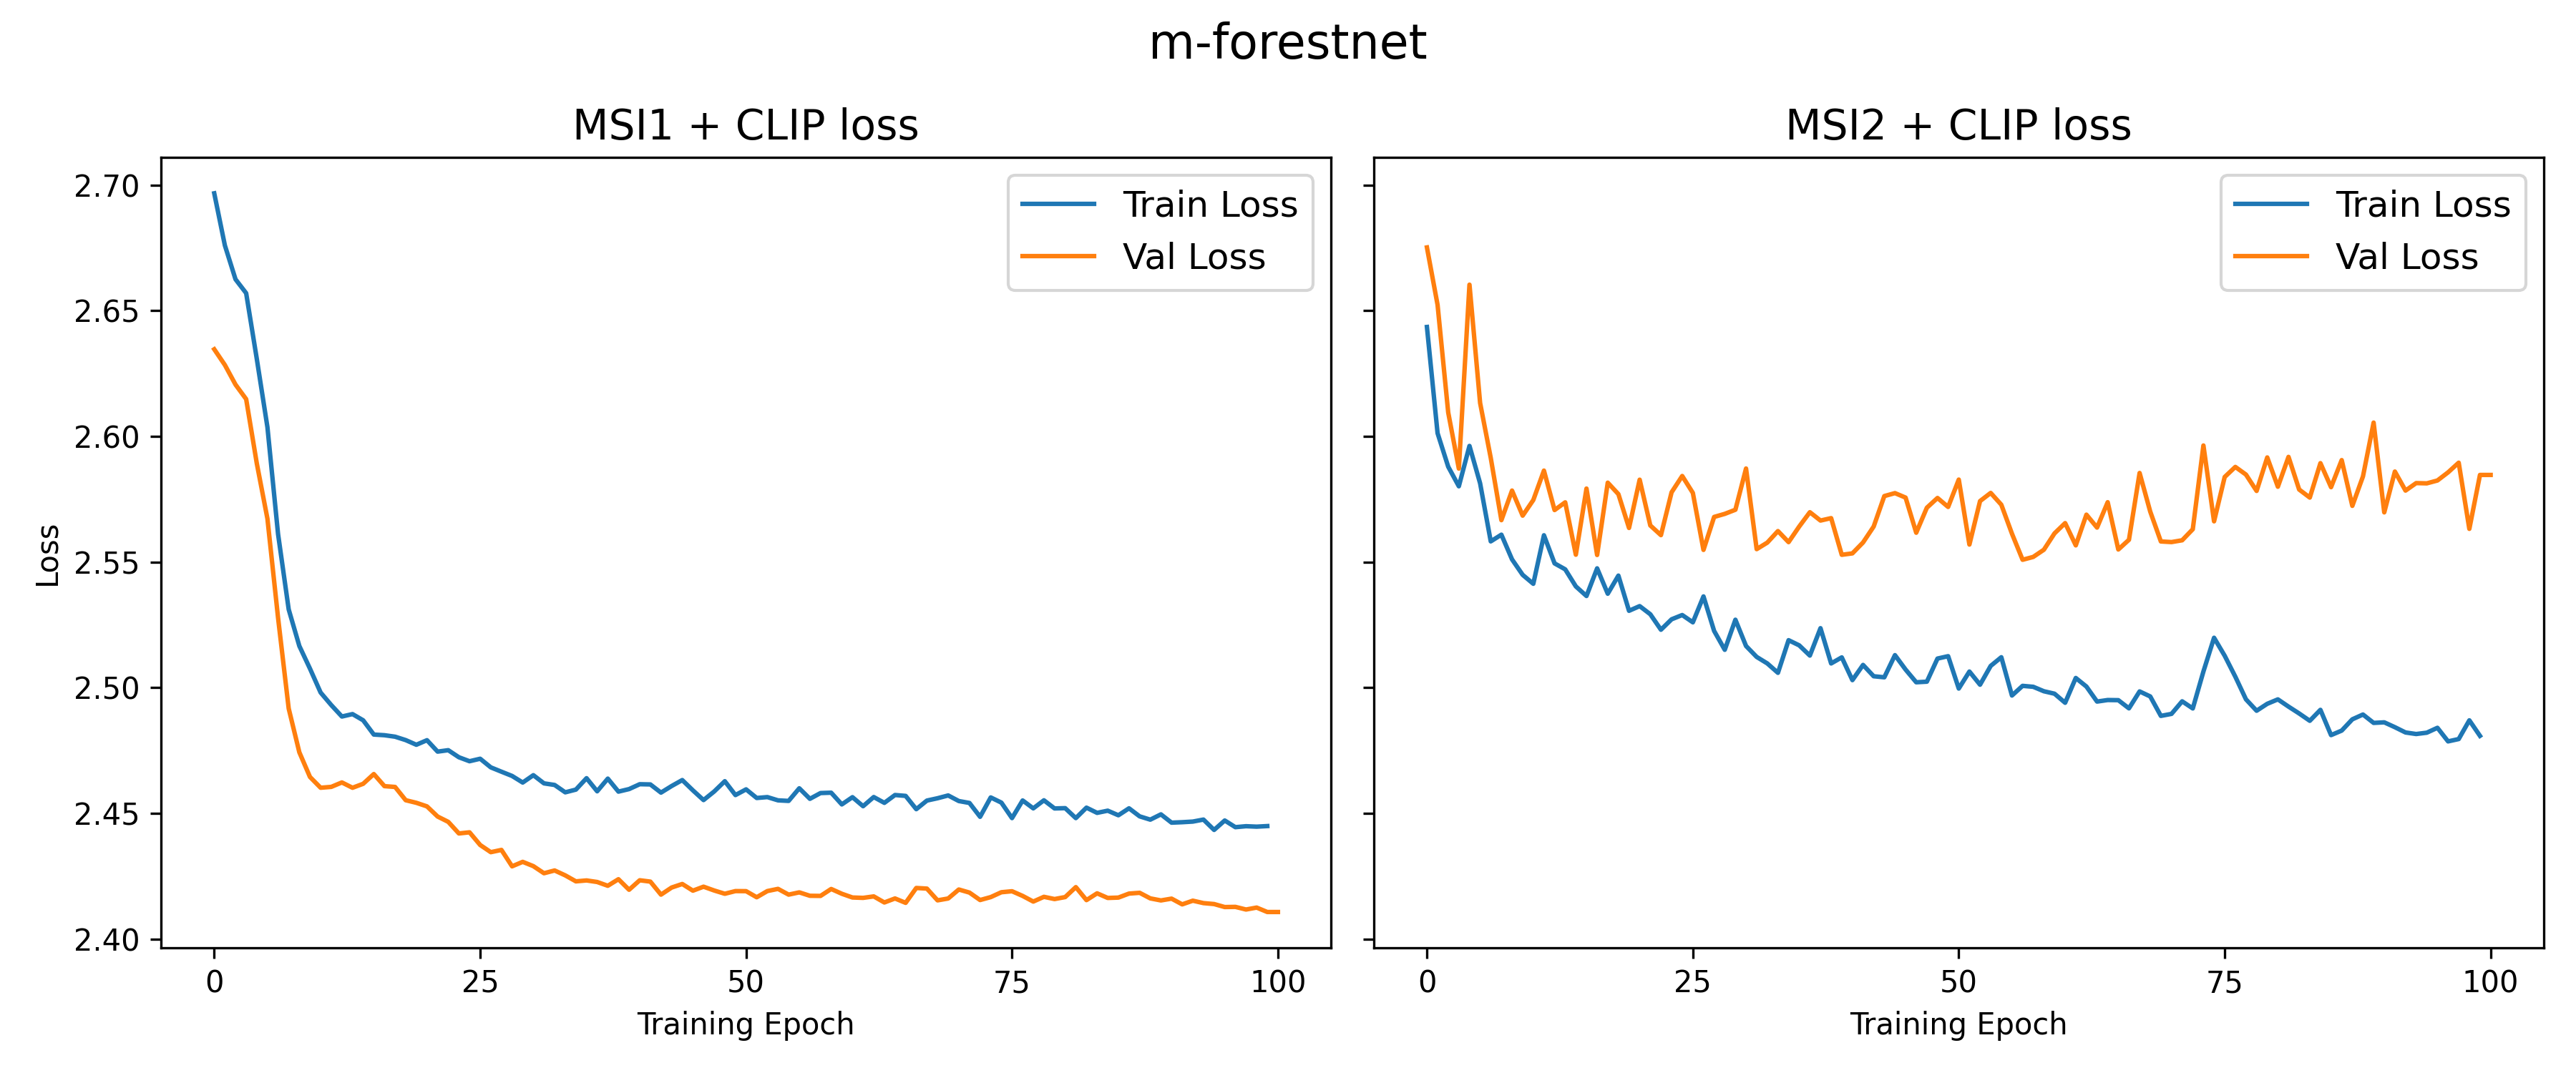
\includegraphics[width=\textwidth]{img/m-forestnet_loss_plot.png}
    \caption{Training and validation loss of the two embedders on the m-forestnet dataset from GEO-Bench.}
    \label{fig:foresloss}
\end{figure}

\begin{figure}[h]
    \centering
    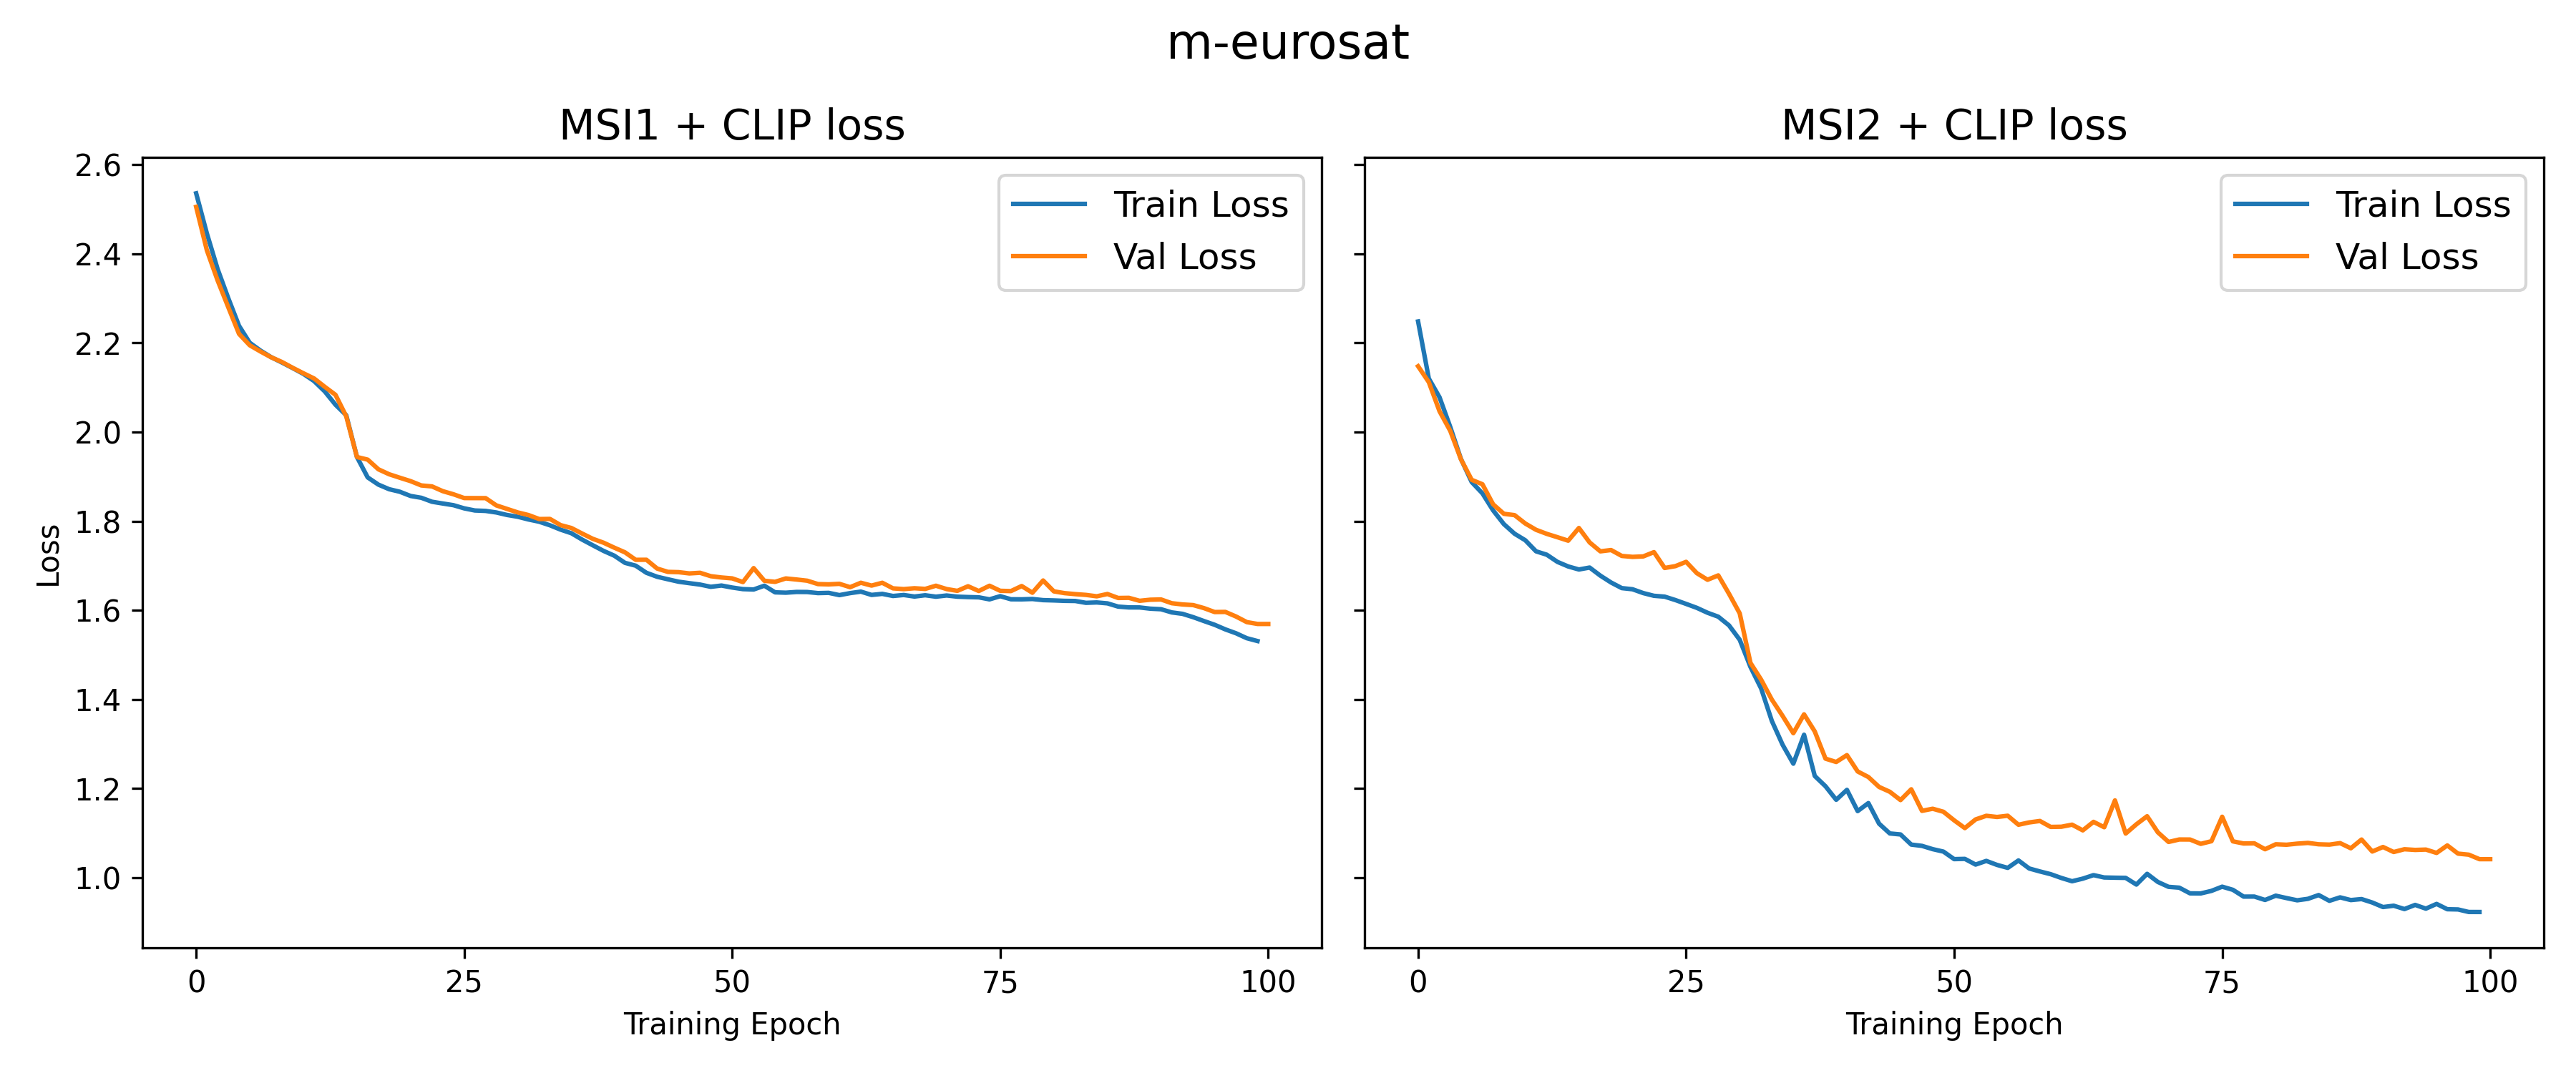
\includegraphics[width=\textwidth]{img/m-eurosat_loss_plot.png}
    \caption{Training and validation loss of the two embedders on the m-eurosat dataset from GEO-Bench.}
    \label{fig:meurosatloss}
\end{figure}

\begin{figure}[h]
    \centering
    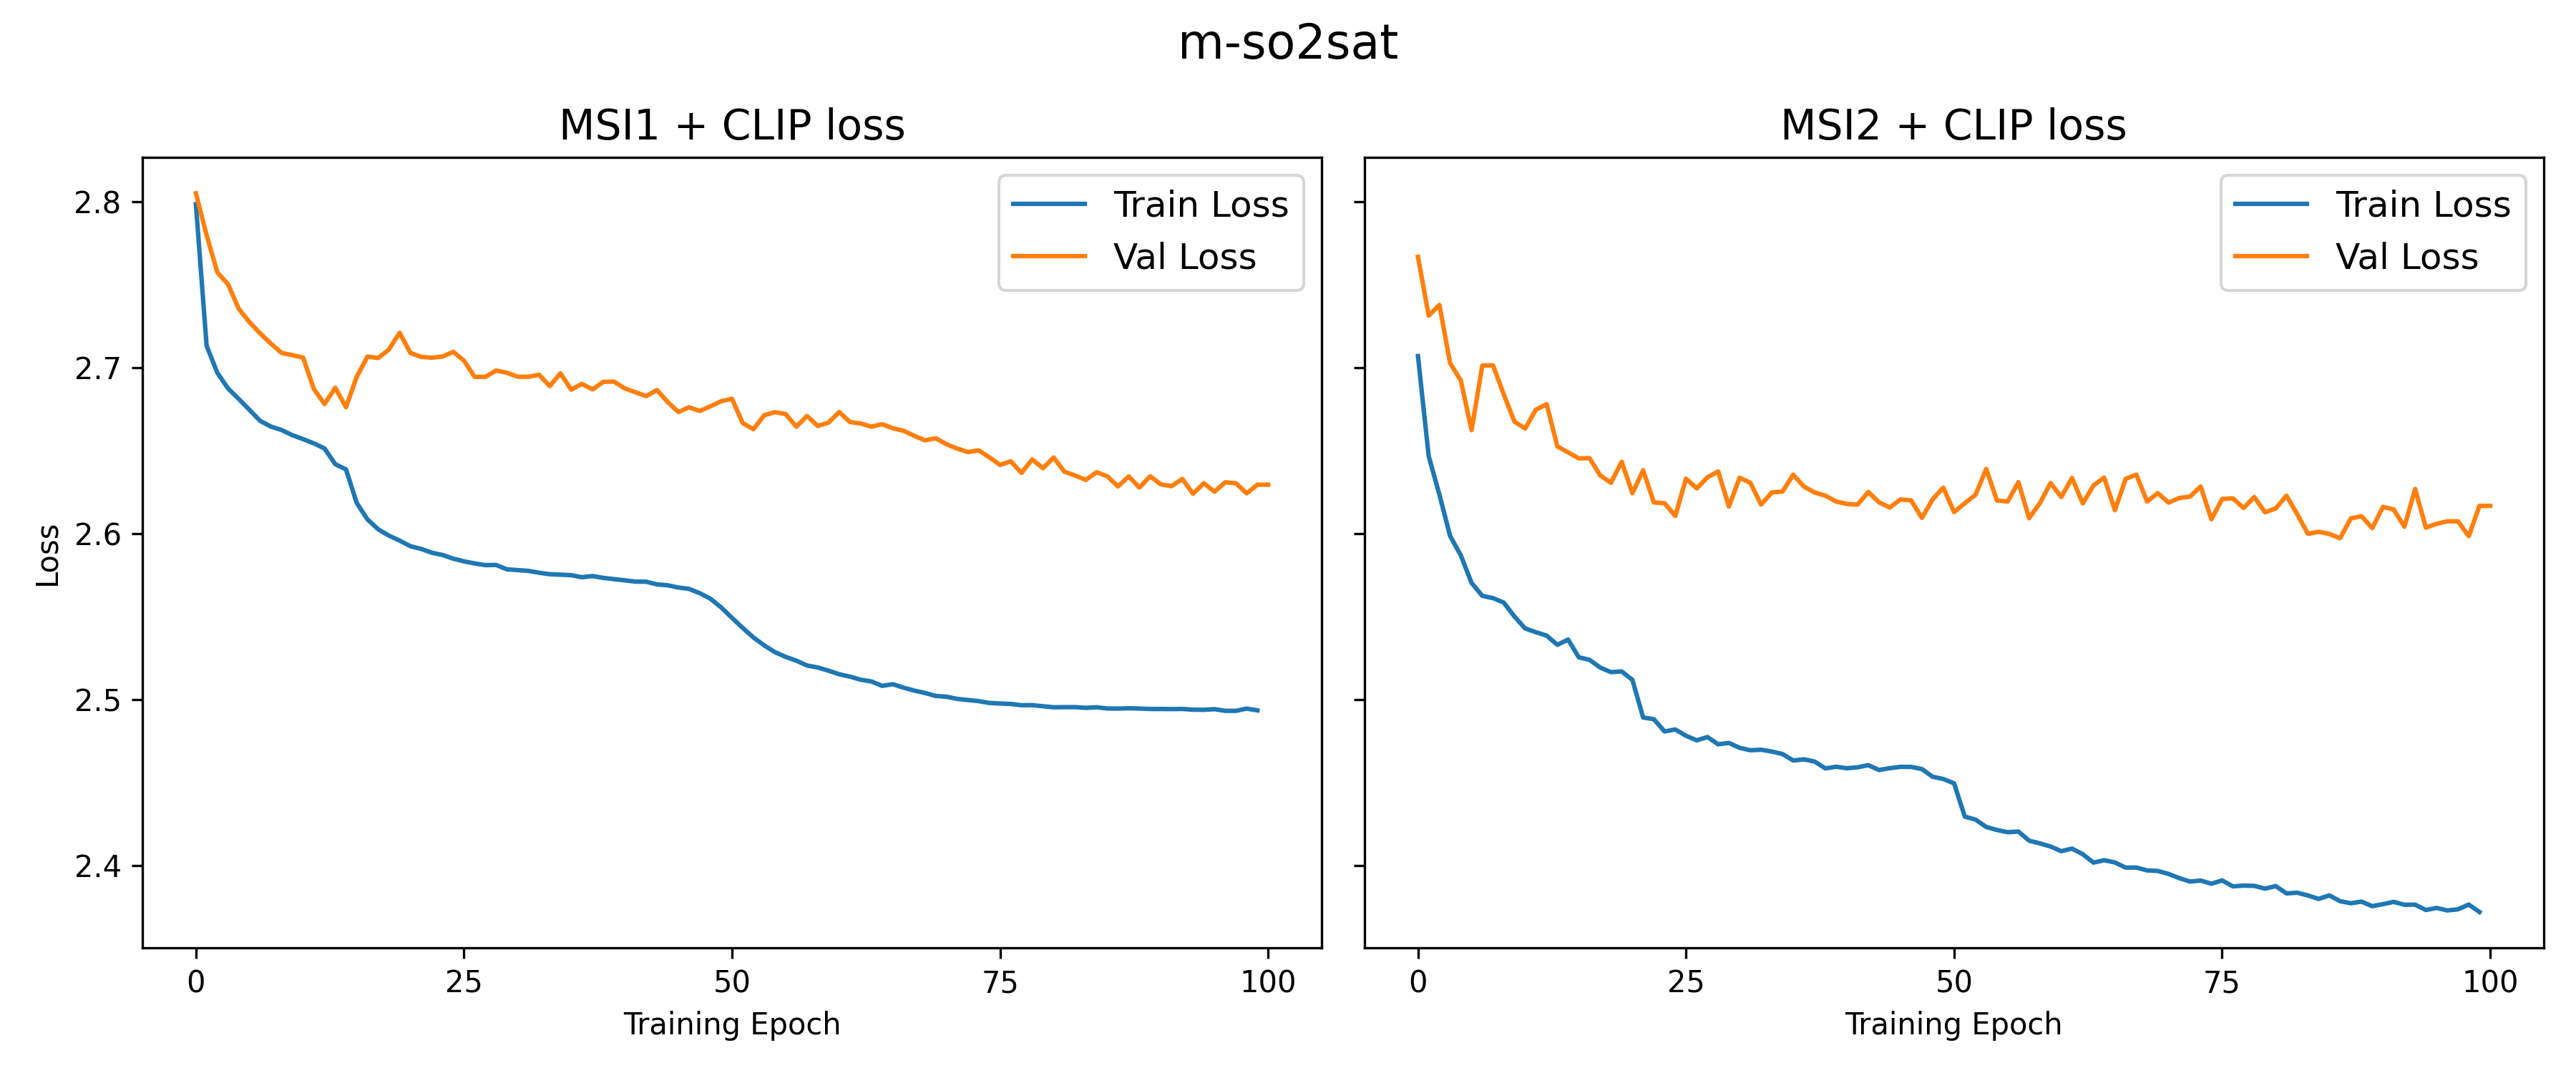
\includegraphics[width=\textwidth]{img/m-so2sat_loss_plot.png}
    \caption{Training and validation loss of the two embedders on the m-so2sat dataset from GEO-Bench.}
    \label{fig:so2satloss}
\end{figure}

\begin{figure}[h]
    \centering
    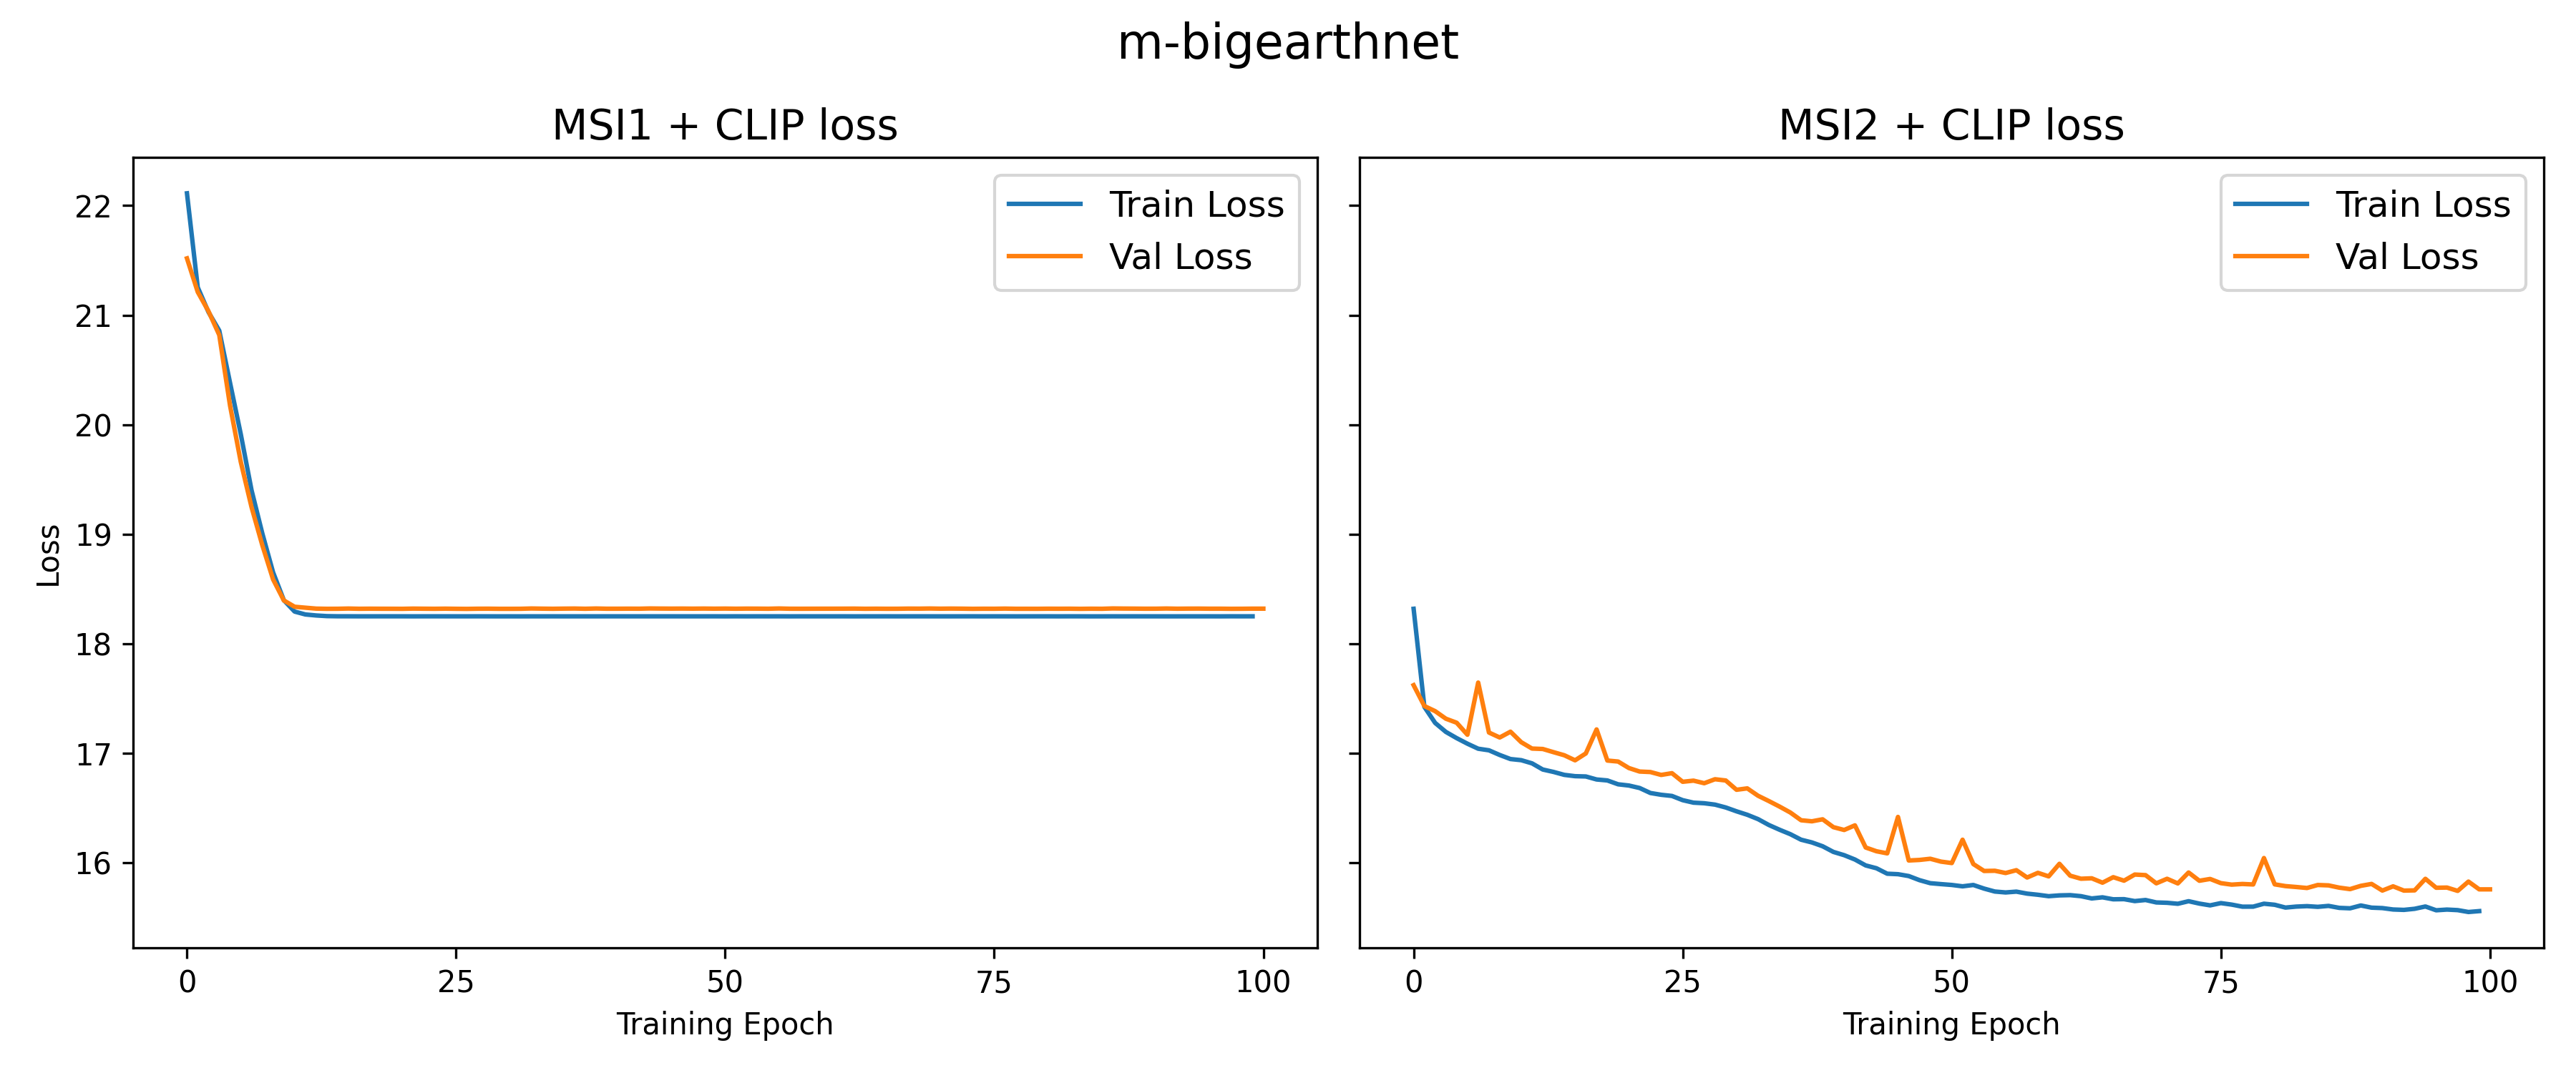
\includegraphics[width=\textwidth]{img/m-bigearthnet_loss_plot.png}
    \caption{Training and validation loss of the two embedders on the m-bigearthnet dataset from GEO-Bench.}
    \label{fig:benloss}
\end{figure}




\chapter{Conclusions} % ---------------------------------------
Conclusions on the work results, discussion of potential future directions (applying the MSI Embedder to a RS-specialized CLIP, trying different models)

Future work directions: hyperparameter tuning, trying bigger embedders, multilabel classification model to be restructured according to what said in that paper (maybe trying something like that with GeoRSCLIP or so, ...

Also see last chapters of the Pi School report


\backmatter
\cleardoublepage

% APPENDIX ----------------------------------------------------
\appendix
\chapter{Appendix}


\begin{table}[ht]
\centering
\footnotesize
\renewcommand{\arraystretch}{1.2}
    \begin{tabular}{cccccc|c}
    \toprule
    %\textbf{Model} & \textbf{Method} & \multicolumn{5}{c}{\textbf{m-bigearthnet}} \\
    \multirow{2}{*}{\textbf{Model}} & \multirow{2}{*}{\textbf{Method}} & \multicolumn{5}{c}{\textbf{m-bigearthnet}} \\
    \cmidrule(lr){3-7}
    & & \textbf{R@5} & \textbf{P@5} & \textbf{mAP} & \textbf{F1} & \textbf{rloss} \\
    \specialrule{.06em}{.2em}{.2em}
    CLIP & zero-shot & \textbf{31.70\%} &  \textbf{23.40\%} & \textbf{32.32\%} & \textbf{20.39\%} & \textbf{28.71\%} \\
    | &  | & | & | & | &| & | \\
    MSI1 & finetune & 19.99\% & 15.58\% & 24.57\% & 15.29\% & 39.82\% \\
    MSI2 & finetune & 15.58\% & 11.46\% & 19.44\% & 14.55\% & 45.53\% \\
    MSI-T-s & zero shot & 15.95\% & 12.84\% & 20.36\% & 16.46\% & 42.26\% \\
    MSI-T-E & zero shot & \underline{29.56\%1} & \underline{22.24\%} & \underline{30.90\%} & \underline{20.30\%} & \underline{28.58\%} \\
    MSI-T-E-4L & zero shot & 24.61\% & 19.02\% & 27.51\% & 19.23\% & 33.45\% \\
    \bottomrule
    \end{tabular}
\vspace{0.3cm}
\caption{\normalsize Performance of models on the m-bigearthnet dataset across various evaluation metrics: the accuracy in bold refers to the best performing model, the underlined one to the second best.}
\label{tab:mbigearthnetresults}
\end{table}


% BIBLIOGRAPHY ------------------------------------------------
\newpage
\phantomsection % use this command only if hyperref is loaded
\addcontentsline{toc}{chapter}{\bibname}
% Here put the code for the bibliography. You can use BibTeX or
% the BibLaTeX package or the simple environment thebibliography.
\bibliographystyle{unsrt} % style can be changed
% 'unsrt' is identical to 'plain', but disables the automatic alphabetical order
\bibliography{references.bib}

\end{document}
